\documentclass[12pt]{article}
\usepackage{longtable}
\usepackage[utf8]{inputenc}
\usepackage[tmargin=1in,lmargin=1in,rmargin=1in]{geometry}
\usepackage{fancyhdr}
\setcounter{tocdepth}{3}
\usepackage{titletoc,tocloft}
\setlength{\cftsubsecindent}{0.65cm}
\setlength{\cftsubsubsecindent}{1.3cm}
\newcommand{\nocontentsline}[3]{}
\let\origcontentsline\addcontentsline
\newcommand\stoptoc{\let\addcontentsline\nocontentsline}
\newcommand\resumetoc{\let\addcontentsline\origcontentsline}
\makeatletter
\newcommand\teenyparagraph[1]{%
  \@tempswatrue
  \if@nobreak\@tempswafalse\fi
  \if@noskipsec \leavevmode \fi
  \par
  \@nobreakfalse
  \everypar{}%
  \protected@edef\@svsec{\@seccntformat{paragraph}}%
  \@tempswafalse
  \@xsect{3.25ex \@plus 1ex \@minus .2ex}%
  {\normalfont\normalsize\bfseries #1}%
}
\makeatother
\usepackage{multicol}
\usepackage{setspace}
\usepackage{graphicx} % Required for inserting images
\usepackage{etoolbox}
\usepackage{pdfpages}
\usepackage{enumitem}
\setlist[itemize]{noitemsep}
\usepackage{listings} % For code listings
\usepackage{color} % For colored text
\usepackage{amsmath} % For mathematical notation
\usepackage{array} % For better table formatting
\usepackage{float}
\usepackage{url}
\patchcmd{\thebibliography}{\section*}{\section}{}{}
\graphicspath{ {./images/} }

\newcommand{\quickimage}[2]{%
\begin{figure}[!htbp]
\centering
\includegraphics[width=#2]{#1}
\end{figure}%
} 

\newcommand{\quickfigure}[4]{%
\begin{figure}[!htbp]
\centering
\includegraphics[width=#2]{#1}
\caption{#3}
\label{#4}
\end{figure}%
} 

\lstset{ %
  numbers=left,           
  stepnumber=1,           
  numbersep=5pt,          
  showspaces=false,           
  showstringspaces=false,     
  showtabs=false,         
  frame=single,           
  tabsize=4,              
  captionpos=b,           
  breaklines=true,            
  breakatwhitespace=false,        
}

\onehalfspacing

\usepackage{subfiles}

%%%%%%%%%%%%%%%%%%%%%%%%%%%%%%%%%%%%%%%%%%%%%%%%%%%%%%%%%%%%%%%%%%%%%%%%%%
%                           Title Page                                   %
%%%%%%%%%%%%%%%%%%%%%%%%%%%%%%%%%%%%%%%%%%%%%%%%%%%%%%%%%%%%%%%%%%%%%%%%%%
\begin{document}

\begin{titlepage}
    \begin{center}
        \raisebox{-0.5\height}{
\includegraphics[width=4cm]{template/Picture2.jpg}} \hfill
        \raisebox{-0.5\height}{
\includegraphics[width=6cm]{template/Picture1.png}} \hfill
        \raisebox{-0.5\height}{
\includegraphics[width=4cm]{template/pki-logo.png}}
        
        {\Large College of Engineering\\
        Electrical and Computer Engineering Department\\}
        
        \vspace{2cm}
        {\Large ECEN 495}
        \vspace{0.5cm}
        
        {\Huge The Harm Drone}
        \vspace{2.5cm}
        
        {\large By\\}
        \begin{Large}
        Carter Brehm \\
        Toby Heinemann \\
        Camryn Klintworth \\
        Michael Maline\\
        \end{Large}
        
        \vspace{2cm}
        
        \small Submitted in Partial Fulfillment of the Requirements for the B.Sc. Degree,\\
        \small Electrical and Computer Engineering,\\
        \small College of Engineering,\\
        \small University of Nebraska-Lincoln,\\
        \small Peter Kiewit Institute, Omaha, Nebraska, U.S.A.\\
        \small May 2025\\
    \end{center}
    \thispagestyle{empty}
\end{titlepage}

\newpage

%%%%%%%%%%%%%%%%%%%%%%%%%%%%%%%%%%%%%%%%%%%%%%%%%%%%%%%%%%%%%%%%%%%%%%%%%%
%                        Front Matter                                    %
%%%%%%%%%%%%%%%%%%%%%%%%%%%%%%%%%%%%%%%%%%%%%%%%%%%%%%%%%%%%%%%%%%%%%%%%%%
\section*{Front Matter}

\subsection*{Ethical Design Statement}
%A statement affirming that the Code of Ethics of the IEEE has been reviewed and applied to the design process and in the selection of the final proposed design. And that, the designers have held the safety of the public to be paramount and have addressed this in their design.
The design and development of the Harm Drone system adhered to the IEEE Code of Ethics throughout the entire engineering process. Under these principles, the team prioritized public safety, transparency, and the responsible use of technology. Key design decisions, such as compliance with IEEE 1789-2015 lighting standards, modular architecture to avoid misuse, and the exclusion of wireless telemetry to minimize privacy and interference concerns, reflect the team's commitment to safety and ethical responsibility. All system features were evaluated for potential misuse, and the final design avoids applications that could compromise human well-being or data integrity. The team remained honest about the limitations of the system and sought guidance from the faculty when needed to ensure that all work upheld professional standards of conduct.

\subsection*{Environmental Impact Statement}
%A statement declaring that the designers have considered any impact to the environment in their design and have eliminated the use of toxic materials, specifically those dangerous to humans.
The Harm Drone was designed with environmental responsibility in mind. All components used in the final product were selected to avoid hazardous substances, per RoHS (Restrictions of Hazardous Substances) guidelines wherever possible. The 3D printed enclosure was made using PLA, a biodegradable thermoplastic derived from renewable resources such as corn starch, minimizing the long-term environmental impact. In addition, the system is powered by rechargeable LiPo batteries, which reduces single-use waste. During development, no toxic materials were introduced, and care was taken to avoid unnecessary component waste. The project’s commitment to sustainability extends to future deployment, where low power consumption and reusability support long-term environmental management.

\subfile{sections/abstract.tex}

\subsection*{Acknowledgement}

Group 127 would like to acknowledge the invaluable support and assistance provided by faculty members of the University of Nebraska.
\teenyparagraph{Dr. Herbert Harms}'s enthusiasm for drone-based research and data collection was what inspired Group 127 to begin the project, and his continued financial support allowed us to deliver a completed product.
\teenyparagraph{Dr. Hamid Sharif}'s lessons on PCB design, architecture, and more specifically, USB communication, were invaluable to the completion of the project.
\teenyparagraph{Prof. Herbert Detloff}'s instruction regarding working as a multi-disciplinary, high-performance engineering team helped us to effectively distribute work, complete milestones, and finalize the project effectively.

%%%%%%%%%%%%%%%%%%%%%%%%%%%%%%%%%%%%%%%%%%%%%%%%%%%%%%%%%%%%%%%%%%%%%%%%%%
%                     Executive Summary                                  %
%%%%%%%%%%%%%%%%%%%%%%%%%%%%%%%%%%%%%%%%%%%%%%%%%%%%%%%%%%%%%%%%%%%%%%%%%%
\newpage
\section*{Executive Summary}

%\subsection*{Foreword}
%\begin{itemize}[noitemsep]
 %   \item Give the problem statement including the organizational problem, (the purpose of capstone projects, the context of your project) and the general technical problem (the type of project you are doing (software prototype, hardware prototype, application program for a client, etc.).
 %   \item Give a more specific assignment statement --- specifically what the writers of the report were asked to do (an overview of the project goals), the technical questions, task, and perhaps the hypothesis or solution.
  %  \item State the overall purpose of the report.
%\end{itemize}

\par The Harm Drone project addresses an organizational and technical gap in the availability of low cost, modular, and platform-independent embedded systems for data collection in small unmanned aerial vehicles (UAVs). As UAVs become increasingly important across sectors such as environmental monitoring, agricultural research, education, and public safety, the need for affordable and reliable onboard computing platforms has become apparent. Commercial systems often impose high costs, proprietary interfaces, and infrastructure requirements, creating barriers for academic institutions and other small research teams. Capstone projects like this one exist to solve such real world engineering problems by guiding students through a complete design process while emphasizing innovation, feasibility, and societal impact.

\par This project was assigned as a capstone senior design challenge within the Electrical and Computer Engineering department. The task was to design, fabricate, and test a cost-effective PCB based embedded system capable of logging data from USB sensors, storing it securely in multiple formats, and integrating into UAV platforms without relying on wireless telemetry. The technical questions included: Can reliable multi sensor data logging be achieved with minimal power consumption and without wireless transmission? Can such a system remain lightweight, durable, and universally accessible across major operating systems? The overarching hypothesis was that a low cost, standards compliant solution could be developed using off the shelf components and open hardware principles without sacrificing functionality or performance.

\par The purpose of this report is to document the design process, engineering tradeoffs, component decisions, packaging considerations, test results, and ethical implications of the Harm Drone system. It serves as both a record of the team’s technical accomplishments and a roadmap for future research teams or developers interested in scalable embedded UAV solutions. This report outlines how an interdisciplinary team transformed a high level design goal into a working, tested product with demonstrated real world potential. It also highlights the nature of requirements in a real engineering project and the importance of adaptability, stakeholder feedback, and iterative refinement in achieving a successful outcome.

\par Through a comprehensive analysis of performance, cost, safety, sustainability, and regulatory compliance, this report provides a complete engineering narrative from problem formulation to final prototype validation. The Harm Drone system not only meets its initial objectives but also offers a scalable foundation for future academic and industrial development.

\subsection*{Summary}
%\begin{itemize}[noitemsep]
   % \item Provide the objective and background (how problem was approached, what were the results) including objective or hypothesis, methodology or experimental procedure and results.
  %  \item Give overall conclusions about the project including recommendations for improvements and their implications, subsequent action, and cost and benefits.
%\end{itemize}

\par The objective of the Harm Drone project was to develop a low cost, modular embedded system that enables UAVs to log high fidelity sensor data without reliance on wireless telemetry. This system needed to operate across various platforms, ensure cross-compatibility with major operating systems, support multiple USB sensors, and comply with lighting safety standards. The technical challenge was approached using an iterative engineering design process that incorporated hardware prototyping, embedded systems development, enclosure fabrication, and rigorous performance validation.

\par The methodology included selecting and integrating key components such as the STM32 microcontroller, USB hubs, EEPROM, LDO regulator(Low Dropout), and a buck converter into a custom PCB. The team also developed firmware to manage real time USB communication and data logging. Testing was conducted to verify data retention, throughput, power consumption, boot time, and lighting compliance. 

\par The overall conclusion of the project is that it is entirely feasible to deliver a UAV compatible data logging platform at a fraction of the commercial cost using open source tools and modular design principles. The Harm Drone system demonstrates that affordability does not have to come at the expense of performance or safety.

\par Recommendations for future improvements include the addition of wireless communication as an optional module, enhanced environmental sealing for field use, and expansion of firmware support for additional sensor types. These changes would further increase the versatility and robustness of the system while maintaining its low cost ethos. The success of this project opens opportunities for further development in academic, environmental, and industrial applications where cost-effective, reliable sensor systems are essential.

%%%%%%%%%%%%%%%%%%%%%%%%%%%%%%%%%%%%%%%%%%%%%%%%%%%%%%%%%%%%%%%%%%%%%%%%%%
%                     Table of Contents                                  %
%%%%%%%%%%%%%%%%%%%%%%%%%%%%%%%%%%%%%%%%%%%%%%%%%%%%%%%%%%%%%%%%%%%%%%%%%%
\newpage
\tableofcontents
\listoffigures
\listoftables
\newpage

%%%%%%%%%%%%%%%%%%%%%%%%%%%%%%%%%%%%%%%%%%%%%%%%%%%%%%%%%%%%%%%%%%%%%%%%%%
%                         Introduction                                   %
%%%%%%%%%%%%%%%%%%%%%%%%%%%%%%%%%%%%%%%%%%%%%%%%%%%%%%%%%%%%%%%%%%%%%%%%%%
\section{Introduction}
%The introduction should orient the reader to the topic of the report by including the following:
%\begin{itemize}[noitemsep]
 %   \item \textbf{The problem} - Explain the problem that is addressed in the report.
 %  \item \textbf{The objective} - State the objectives (what your project needs to accomplish to solve the problem).
 %   \item \textbf{The method of the report} - Describe the organization and structure of the report.
%\end{itemize}
\subsection{Problem Statement}

\par As unmanned aerial vehicles (UAVs) become more accessible and widely used across industries such as environmental monitoring, scientific research, and education, the need for affordable, reliable onboard computing and data acquisition systems has grown significantly. However, many existing drone platforms are constrained by high costs associated with proprietary sensor interfaces, specialized data acquisition modules, and storage systems that require additional licensing, software, or support infrastructure. These factors create financial barriers for small teams, educational institutions, and low budget field operations.

\par A core issue lies in the lack of a cost-effective, standardized, and platform independent onboard system capable of collecting high fidelity sensor data in real time, storing it securely for later analysis, and operating without dependence on expensive or wireless infrastructure. Many current solutions rely on wireless telemetry, which not only increases cost but also introduces the risk of signal interference, data loss, and added complexity especially in remote or resource limited environments. Furthermore, data stored using proprietary formats often requires extensive post processing or specialized software, increasing both time and cost for analysis.

\par Safety considerations also factor into cost conscious designs. For example, compliance with IEEE 1789-2015 lighting standards is important for human safety and public deployment, yet many low cost drone systems overlook these features due to the expense and complexity of implementation. The absence of safe, flicker free lighting can limit where and how these drones can be used.

\par The Harm Drone project addresses these problems by designing and prototyping a universal, low cost drone mounted PCB system. The design supports USB connected sensors eliminating the need for expensive custom interfaces and features high capacity SD card storage for offline data collection, readable across all major operating systems. Data integrity is preserved using onboard nonvolatile memory, removing the need for costly real time transmission. Additionally, the system incorporates a lighting subsystem compliant with IEEE flicker safety guidelines, balancing affordability with safety. By eliminating the reliance on expensive, proprietary, or wireless systems, The Harm Drone aims to deliver a practical, scalable solution for researchers, developers, and educators working within constrained budgets.

\subsection{Project Objectives}

\par The Harm Drone project seeks to provide a functional and affordable embedded platform tailored to the unique requirements of UAV based research and data collection. The primary objective is to design a universal sensor interface and data logging system that minimizes cost while maximizing utility, modularity, and safety. In pursuit of this goal, the project sets forth the following expanded objectives:

\begin{itemize}
\item \textbf{Affordability:} Develop a complete PCB system that meets all functionality goals with a total materials cost under \$420, allowing academic and low budget users to adopt the technology without financial strain.

\item \textbf{Sensor Modularity:} Enable plug and play compatibility with up to four USB based sensors. This allows end users to customize data collection based on mission specific needs without modifying firmware or hardware.

\item \textbf{Platform Independence:} Ensure compatibility with diverse UAV platforms and data workflows by using universal interfaces, standard power connections, and a removable SD card formatted in FAT32. This approach reduces setup time and simplifies integration across different systems.

\item \textbf{Persistent, Redundant Storage:} Provide dual layer data storage through onboard flash and removable SD cards, ensuring that valuable data is not lost due to system resets, power failure, or improper shutdown.

\item \textbf{User Accessibility:} Design an intuitive and self documenting file storage structure for data logs to reduce post-processing time and avoid dependency on proprietary decoding tools.

\item \textbf{Regulatory Compliance:} Implement a PWM lighting system that complies with IEEE 1789-2015 flicker safety standards to protect human observers and expand use in public or safety critical environments.

\item \textbf{Ease of Manufacture and Repair:} Use through hole and standard surface mounting components wherever feasible to facilitate assembly and field repairs. The board layout also prioritizes accessibility and isolation of high current paths from logic circuits.

\item \textbf{Rapid Deployment and Boot Time:} Ensure the system is flight ready in under 5 seconds from power on, reducing operational downtime and maximizing mission uptime.

\item \textbf{Durability and Protection:} Package the PCB in a 3D printed PLA enclosure that is lightweight, impact resistant and modular. The enclosure design allows for quick access to ports and simplifies part replacement.

\item \textbf{Environmental Responsibility:} Prioritize sustainable materials, minimize power consumption, and enable responsible disposal at end of life.

\end{itemize}

\par Collectively, these objectives define the technical, operational, and ethical framework of the Harm Drone system. They were informed by a decision weighted objective tree analysis, which helped the team prioritize features that maximized functionality under strict budget constraints. For example, USB sensor compatibility and removable storage were assigned high weight in the decision-making process due to their influence on system modularity and accessibility. Meanwhile, regulatory compliance and ease of use contributed to the system's broader applicability in public, academic, and environmental contexts. This structured evaluation ensured that all objectives aligned with the core mission of delivering a research grade, cost conscious PCB system for UAV deployment. They serve as the foundation for all subsequent design, testing, and validation activities outlined in the remainder of this report.

\subsection{Method of the Report}

\par This report is organized to reflect the complete engineering design cycle and evaluation process of the Harm Drone system. Each section is developed to provide clarity, depth, and rationale for the decisions made by the team throughout the course of the project. The structure of the report is as follows:

\begin{itemize}
\item \textbf{Section 2: Problem Definition and Formulation} \newline
Describes the design context, the evolving nature of system requirements, competitive analysis, and how our team formulated the design problem.

\item \textbf{Section 3: Design Requirements, Specifications, and Success Criteria} \newline
Presents a comprehensive table of performance specifications, the criteria used to define success, and how they align with course defined deliverables.

\item \textbf{Section 4: Concept Development and Design Process} \newline
Includes the literature review, concept generation and reduction processes, production timeline, and engineering tradeoffs.

\item \textbf{Section 5: Detailed Engineering Analysis and Design Product Presentation} \newline
Contains a detailed description of the final PCB layout, packaging, and power design. This section also includes estimated and actual performance metrics.

\item \textbf{Section 6: Economic Analysis} \newline
Provides the cost of the prototype, labor estimates, bill of materials, and economic feasibility of future expansion.

\item \textbf{Section 7: Reliability and Safety Analysis} \newline
Explains hazard analysis and safety validation methods applied throughout the design.

\item \textbf{Section 8: Social, Political, and Environmental Impact} \newline
Discusses ethical implications, regulatory compliance, lifecycle sustainability, and how the system aligns with professional engineering standards.

\item \textbf{Section 9: Conclusions and Recommendations} \newline
Summarizes results, lessons learned, and suggests areas of future improvement.

\item \textbf{Section 10: User Manual} \newline
A comprehensive guide to installing, configuring, and maintaining the Harm Drone PCB.

\item \textbf{Section 11: Appendices} \newline
Includes schematics, flowcharts, timing diagrams, software listings, safety checklists, and other supporting documentation.

\end{itemize}

By following this structure, the report ensures clarity for both technical and non-technical audiences while providing deep insight into our engineering process. The Harm Drone design exemplifies how a small student led team can develop a complex embedded system with real world utility and academic value.



%%%%%%%%%%%%%%%%%%%%%%%%%%%%%%%%%%%%%%%%%%%%%%%%%%%%%%%%%%%%%%%%%%%%%%%%%%
%                    Problem Formulation                               %
%%%%%%%%%%%%%%%%%%%%%%%%%%%%%%%%%%%%%%%%%%%%%%%%%%%%%%%%%%%%%%%%%%%%%%%%%%
\section{Problem Formulation}
\subsection{Problem Statement}
%State the problem to be solved as indicated by the need (the university, industry sponsor, or self-proposed). Present the objectives and expectations of the need and constraints given to the problem.
\par In many academic and research applications, there is a growing demand for reliable and cost-effective unmanned aerial systems (UAS) capable of collecting and storing high fidelity environmental or system data. However, current drone systems used in industry and academia frequently rely on expensive proprietary sensors, specialized storage modules, and wireless transmission protocols that are not only costly, but also introduce reliability risks in field conditions. The result is a significant barrier to entry for budget conscious research teams, student projects, and field operations requiring autonomy, robustness, and open platform support.

\par The problem, therefore, is to design a universal low cost data acquisition and logging system for drones that supports modular integration of USB sensors, data storage onboard with integrity verification, and compliance with operational safety standards. The solution must not rely on wireless data transmission, must store data in a platform agnostic format, and must be rugged enough for field deployment in moderate outdoor environments.

\par This project is self proposed and sponsored by the University of Nebraska Omaha in partial fulfillment of capstone design requirements. The expectations include delivering a working prototype that meets five measurable criteria (PSSCs), including USB sensor interfacing, SD card compatibility, nonvolatile memory recovery, IEEE 1789-compliant lighting, and successful cross-platform data retrieval. Constraints include a fixed budget of \$420, a maximum PCB size compatible with most hobby grade drones (100mm x 100mm), and delivery by the designated final demonstration date.

\subsection{Background}
%Discuss the state of the art, competitive products, and patent liability analysis (HW 1).

\par Modern UAV applications span a wide range of fields, from agriculture and precision mapping to environmental monitoring, disaster response, and research support. In each case, data collected from sensors onboard the UAV is critical to the mission's success. Currently, many commercial UAVs use integrated, non-modular systems or require high end payloads with proprietary interfaces (e.g., DJI’s XT2 or Micasense multispectral sensors), which cost hundreds to thousands of dollars. These products often include limited options for local data storage, requiring operators to rely on wireless links such as Wi-Fi, LTE, or proprietary telemetry protocols. While effective under certain conditions, these links can become unstable or entirely unusable in remote environments or electromagnetically noisy regions.

\par Academic UAV platforms such as ArduPilot-based systems, Raspberry Pi drones, or Pixhawk-integrated quadcopters—do allow for open-source development and hardware extension. However, most lack standardized USB sensor interfacing, relying instead on I2C, SPI, or UART protocols. Integrating external sensors often requires deep firmware changes and power conversion boards, further increasing complexity and cost. Moreover, these systems rarely include robust data integrity checking, making them vulnerable to power loss or in flight resets.

\par In terms of lighting systems, few small UAVs incorporate flicker safe lighting. IEEE Standard 1789-2015 was developed to address biological risks associated with pulse width modulated (PWM) light sources—especially those visible to human observers or operating in environments where safety and compliance are essential. While this standard is widely used in lighting and display engineering, it is largely ignored in hobby and research drone lighting systems due to added cost and design complexity.
\par As these challenges and gaps in current UAV systems became evident, it was necessary to explore the existing commercial landscape and intellectual property space to understand where our system could differentiate itself—both technologically and legally. A formal review of patents and competitive products was conducted to identify potential overlaps, draw inspiration from existing solutions, and ensure that \textit{The Harm Drone} does not infringe upon established claims or technologies.

\subsubsection{Results of Patent and Product Search}

\par To assess potential patent infringement risks for \textit{The Harm Drone}, it is essential to examine existing patents with similar functions. One of the most relevant is \textbf{US 11,501,483 B2}, \textit{Removable Sensor Payload System for Unmanned Aerial Vehicle Performing Media Capture and Property Analysis}, filed on November 15, 2022 \cite{speasl2022payload}. This patent describes a modular payload system that allows UAVs to swap sensors for media capture and automated aerial data collection. Given \textit{The Harm Drone}’s use of specialized sensors for autonomous data collection, there is a potential overlap, particularly in sensor payload design and data acquisition methods. To mitigate risks, \textit{The Harm Drone} must ensure its sensor integration does not replicate this removable payload system.

\par Another relevant patent is \textbf{US 2022/0404273 A1}, \textit{High-Altitude Airborne Remote Sensing}, published on December 22, 2022 \cite{kendall2022remote}. This patent describes high-altitude UAVs equipped with specialized sensors for environmental monitoring, where collected data is processed and transmitted to a ground station. \textit{The Harm Drone} operates at lower altitudes, but it shares key functionalities such as autonomous navigation, environmental data collection, and onboard processing. The risk of infringement exists if \textit{The Harm Drone}’s sensor integration and data handling closely resemble those in this patent.

\par Finally, \textbf{US 10,462,366 B1}, \textit{Autonomous Drone with Sensor}, granted on October 29, 2019 \cite{bart2019autodrone}, describes a drone based monitoring system that continuously collects data, even while charging. It integrates stationary ground sensors with drone captured data for real time property surveillance and analysis. Key claims include sensors for monitoring, data collection while docked, and integration with stationary sensors. \textit{The Harm Drone} also incorporates data sensors for environmental monitoring, posing a potential overlap in data collection, processing, and storage. However, \textit{The Harm Drone} does not perform continuous data capture while stationary, reducing the likelihood of direct infringement.

\par By differentiating its sensor integration, flight altitude, and data processing methods, \textit{The Harm Drone} can mitigate potential patent risks while maintaining its research focused functionality.

\subsubsection{Analysis of Patent Liability}

\par To assess \textit{The Harm Drone}'s potential for patent infringement, we examine both \textit{literal infringement} and infringement under the \textit{doctrine of equivalents} concerning US 11,501,483 B2 \cite{speasl2022payload}, US 2022/0404273 A1 \cite{kendall2022remote}, and US 10,462,366 B1 \cite{bart2019autodrone}. While \textit{The Harm Drone} shares functional similarities with these patents, significant differences in design, operation, and data collection methods reduce the likelihood of infringement.

\begin{itemize}
    \item \textbf{US 11,501,483 B2}: Describes a removable sensor payload system for UAVs, allowing modular sensor integration for media capture and property analysis. While \textit{The Harm Drone} also integrates specialized sensors, its design does not use interchangeable payloads but instead features fixed sensors for research applications. Additionally, it focuses on environmental monitoring rather than media capture or property analysis. Under the doctrine of equivalents, despite both projects involving sensor equipped UAVs, \textit{The Harm Drone} prioritizes weather resistance and research driven sensor integration, reducing infringement risks.

    \item \textbf{US 2022/0404273 A1}: Covers high altitude UAV remote sensing with drones designed for real time environmental monitoring. \textit{The Harm Drone}, however, operates at low to mid altitudes and relies on offline data storage rather than live transmission. Under literal infringement analysis, it does not match the altitude dependent and real time features of this patent. Under the doctrine of equivalents, differences in mission profile and data handling further distinguish the project.

    \item \textbf{US 10,462,366 B1}: Details an autonomous drone that collects image data continuously, even while docked. While \textit{The Harm Drone} uses an image sensor, it does not support continuous monitoring or stationary data capture. Instead, it only captures data during pre programmed flight paths. Under both literal infringement and the doctrine of equivalents, the project's scientific and non-surveillance objectives offer meaningful differentiation.
\end{itemize}

\par In conclusion, \textit{The Harm Drone} is unlikely to literally infringe any of these patents due to differences in operational design, sensor integration, and data processing. While conceptual similarities exist in UAV based data collection, distinctions in implementation and objectives further reduce patent conflict risks.

\subsubsection{Action Recommended}

\par To further mitigate patent infringement risks, \textit{The Harm Drone} should prioritize structural and operational differentiation rather than simply adding new features. Key recommendations include:

\begin{itemize}
    \item \textbf{Sensor Integration:} Avoid modular or swappable sensor payloads as described in US 11,501,483 B2. Fixed or semi-permanent sensor mounting and hardwired connections are preferred. Custom connectors rather than universal mounts will further distinguish the system.
    
    \item \textbf{Altitude and Transmission Constraints:} Operate strictly within low to mid altitude ranges and avoid any real time data transmission to differentiate from US 2022/0404273 A1. Offline storage and post flight data retrieval should be emphasized.

    \item \textbf{Custom Software and Algorithms:} Develop custom navigation and flight control software, rather than depending on proprietary or lightly modified open source frameworks. This avoids infringing on patented control algorithms or autonomous behaviors.

    \item \textbf{Research Positioning:} Clearly brand and document \textit{The Harm Drone} as a tool for environmental research or agricultural data collection. Avoid surveillance, property monitoring, or media capture use cases to limit overlaps with broad UAV surveillance patents.
\end{itemize}

\par By implementing these strategic modifications—including non-removable sensor integration, altitude and data handling restrictions, waypoint bound data collection, and unique flight software—\textit{The Harm Drone} will remain functionally distinct from the referenced patents. These actions will protect the project from infringement risk while achieving its design goals.
\par With a clear understanding of existing patent landscapes and actionable steps to avoid infringement, the focus of the project now shifts from legal differentiation to technical implementation. These patent driven constraints directly inform the design problem, shaping both the hardware and software requirements. In the following section, the core engineering challenge is formally defined, incorporating key limitations such as non-removable sensors, offline operation, and standards compliance. This formulation ensures that the project not only avoids legal conflicts but also addresses real world needs for robust, low cost UAV data systems.

\subsection{Problem Formulation}
%Show that the problem has been formulated by presenting appropriate design method objectives, taking into consideration the following factors:
%\begin{itemize}[noitemsep]
   % \item (a) Problem is realistic or satisfies a specified need
   % \item (b) Easy to verify and/or validate by the end of the project
%\end{itemize}

\par To address the limitations of current UAV data systems, this project formulates a hardware and software co-design problem centered around developing a cost-effective, modular, and platform independent onboard computing solution. The core engineering challenge is to design a drone compatible embedded system capable of collecting sensor data from multiple sources, storing that data in a portable format, and maintaining operational reliability under autonomous, offline conditions—all while staying within a limited budget and adhering to safety standards.

\par This problem is realistic and addresses a well defined need within both academic and applied research domains. Many existing UAV platforms used in environmental monitoring, fieldwork, or educational applications lack modular sensor integration, support only proprietary or complex communication protocols, and often rely on unreliable wireless transmission methods. These limitations significantly restrict accessibility for small teams, educators, and research groups working with limited financial and technical resources.

\par The formulated design problem requires the development of a compact embedded system that:
\begin{itemize}
    \item Communicates with multiple external sensors using standard, low cost interfaces;
    \item Collects and stores high resolution environmental data during flight;
    \item Maintains data integrity in the event of unexpected power loss;
    \item Stores collected data in a format readable across all major operating systems;
    \item Integrates a safety compliant lighting system suitable for use around people;
    \item Operates without reliance on a wireless connection or cloud based infrastructure;
    \item Remains compact, lightweight, and compatible with common UAV platforms.
\end{itemize}

\par The design method is structured to satisfy both engineering feasibility and verification at each stage of development. The system architecture must remain adaptable for testing under simulated or real UAV flight conditions, allowing for validation of each subsystem independently—such as power management, data handling, interface timing, and sensor communication. Design constraints related to size, power consumption, and data compatibility are selected specifically to ensure that the final product can be verified through bench testing, field simulation, and cross-platform data access.

\par This problem formulation enables an iterative design approach, incorporating hardware prototyping, embedded firmware development, and system level validation. By focusing on modularity, offline data handling, and cross-platform accessibility, the project remains grounded in realistic engineering constraints while offering meaningful impact in real world applications such as environmental monitoring, agriculture, and research support.
\par To translate this problem formulation into an actionable engineering plan, a detailed set of design requirements and specifications must be established. These specifications form the foundation for evaluating the success of the final system and ensure that all subsystems align with both project goals and external constraints, such as compliance standards and operational environments. By defining clear, quantifiable metrics, the design team can track progress, validate subsystem performance, and verify that the integrated system meets all functional and safety expectations. The following section outlines these specifications, along with the criteria that will be used to determine whether the project successfully achieves its technical objectives.

%%%%%%%%%%%%%%%%%%%%%%%%%%%%%%%%%%%%%%%%%%%%%%%%%%%%%%%%%%%%%%%%%%%%%%%%%%
%    Project Design Requirements, Specifications, and Success Criteria     %
%%%%%%%%%%%%%%%%%%%%%%%%%%%%%%%%%%%%%%%%%%%%%%%%%%%%%%%%%%%%%%%%%%%%%%%%%%
\section{Project Design Requirements, Specifications, and Success Criteria}
%\begin{itemize}[noitemsep]
  %  \item Give a clear set of design specifications for the project. The design specifications should be clear concise statements with a specific metric and an appropriate value.
  %  \item The specifications should provide an unambiguous measure of the success of the final design in meeting the need and constraints associated with the design problem.
  %  \item Problem Requirements Specifications is a dynamic process. Although it is desirable to freeze a set of requirements permanently, it is rarely possible. Requirements are likely to evolve through an iterative process that involves communication between the customer specifying the need and the technical community. The impact of proposed requirements must be evaluated to ensure that the initial intent of the requirements baseline is maintained or that changes to the intent are understood and accepted by the customer. The following diagram summarizes the dynamic process of developing system requirements:
%\end{itemize}

%\begin{center}
%Need or Customer \\
%Developed System Requirements \\
%Design Team Environment/Constraints \\

\par To ensure the solution is viable, measurable, and aligned with real world constraints, this section outlines the detailed design specifications, the success criteria adopted throughout the design lifecycle, and the iterative nature of requirement refinement.

\subsection{Design Specifications}

\par The design specifications for the Harm Drone system establish the functional and physical boundaries necessary for successful operation. These parameters provide measurable criteria for subsystem performance, enabling objective testing, validation, and refinement throughout the development process. Each specification is tied to a quantifiable metric and is supported by a clear rationale.

\begin{table}[H]
\centering
\begin{tabular}{|c|p{3cm}|p{3cm}|p{3cm}|p{4cm}|}
\hline
\textbf{Spec ID} & \textbf{Description} & \textbf{Metric} & \textbf{Target Value} & \textbf{Rationale} \\
\hline
DS1 & Onboard data retention & Data capacity & $\geq$ 1000 KB & Ensures retention of flight, log, and sensor data in persistent memory. \\
\hline
DS2 & Data accessibility & Cross-platform compatibility & Readable on Mac OS, Windows, Debian Linux & Guarantees log access on all major OS platforms. \\
\hline
DS3 & External storage capacity & SD card storage & $\geq$ 4 GB & Provides space for extended data logging. \\
\hline
DS4 & USB sensor support & Concurrent USB connections & Up to 4 sensors & Supports flexible external sensing integration. \\
\hline
DS5 & Light system compliance & Flicker modulation testing & Pass IEEE 1789-2015 check & Meets industry lighting safety standards. \\
\hline
DS6 & PCB fabrication & Trace and via tolerance & $\leq \pm$5 mil & Ensures manufacturability and reliability. \\
\hline
DS7 & USB data throughput & Data transfer rate & $\geq$ 12 Mbps & Enables real time sensor data exchange. \\
\hline
DS8 & Firmware robustness & Uptime with full load & $\geq$ 8 hours & Confirms system stability. \\
\hline
DS9 & Boot time & Power on to readiness & $\leq$ 5 seconds & Improves responsiveness. \\
\hline
DS10 & System packaging & Enclosure volume & $\leq$ 900 cm$^3$ & Ensures drone compatibility. \\
\hline
\end{tabular}
\caption{Project Design Specifications for Harm Drone System}
\end{table}

\par Within the UAV design context, the specifications address environmental, technical, and regulatory considerations. For example, DS1, which concerns onboard data retention, is essential for UAVs operating in remote or disconnected areas where real-time data transmission may be unreliable or impossible. Ensuring robust local storage safeguards mission-critical data, even during unexpected power interruptions.

\par Specifications DS2 and DS3 emphasize interoperability and ease of access. In real-world deployments involving multiple users and varied systems, the ability to seamlessly retrieve data across different operating systems—without requiring extra drivers or file conversions—simplifies analysis and enhances usability. These features align with user-centric design principles.

\par DS4 and DS7 focus on system performance. Since the Harm Drone must interface with multiple sensors simultaneously, the embedded system must support USB 2.0 data rates capable of handling concurrent real-time data streams. These requirements prevent communication bottlenecks and ensure all peripherals operate without interference or data loss.

\par DS5 underscores the project's adherence to health and safety guidelines, particularly the IEEE 1789-2015 standard for minimizing adverse effects caused by LED flicker. Compliance with this standard not only ensures safer operation in human environments but also contributes to an overall higher standard of system usability.

\par DS6 and DS10 address design manufacturability and platform compatibility. Meeting precise fabrication tolerances (DS6) enhances PCB reliability and electrical performance, while adhering to enclosure volume constraints (DS10) guarantees that the system integrates cleanly into standard UAV frames without structural modifications.

\par Lastly, DS8 and DS9 reflect the system’s robustness and responsiveness. A drone that can sustain prolonged operation under full load (DS8) and reboot quickly (DS9) is essential for field deployment scenarios. These characteristics bolster mission readiness and reinforce user confidence in the system’s dependability.

\subsection{Project Common Success Criteria (PCSC)}

\par The Project Common Success Criteria (PCSCs) reflect the core engineering and documentation milestones the team must achieve to ensure comprehensive and professional design execution. These are milestone based and form the checkpoints by which development maturity is assessed.

\par The project success criteria outline a comprehensive approach to ensure the design and implementation of the project meet high quality standards. The first step is to create a complete bill of materials (BoM) that lists all the components required for the design, followed by ordering or sampling these parts to ensure their availability for the development process. This ensures that the project has all the necessary resources to proceed without delays. 

\par The second step involves developing a complete, accurate, and readable schematic of the design, which is essential for visualizing the system’s structure and functionality. This schematic will include detailed analyses such as interface loading analysis to ensure that components can handle their respective loads and interface timing analysis to guarantee that data and signals flow seamlessly across the system without delays or errors.

\par The third step focuses on creating a layout for the printed circuit board (PCB) based on the schematic, followed by etching the PCB to bring the design to life in hardware form. This step ensures the physical implementation of the design is precise and aligns with the schematic. 

\par The fourth step involves populating the PCB with all the necessary components and debugging the design to identify and resolve any issues that may arise during testing, ensuring the final product performs as intended. Lastly, the project will conclude with the professional packaging of the finished product, ensuring that it is not only functional but also presentable. This step will include demonstrating the functionality of the design to validate that it meets the project's objectives and requirements, providing a robust and reliable solution. These criteria ensure a structured and thorough approach to delivering a high quality and successful project.

\begin{enumerate}
    \item \textbf{Complete Bill of Materials:} A detailed and ordered BoM including part numbers, vendor sources, unit costs, and sourcing status. All parts must be either sampled or procured before prototyping.
    \item \textbf{Design Schematic:} A complete schematic with legible labels, interface specifications, and timing analysis. All communication interfaces should be clearly routed and annotated.
    \item \textbf{PCB Fabrication:} Generation and validation of Gerber files. The PCB must meet minimum fabrication tolerances and undergo electrical continuity testing.
    \item \textbf{Board Assembly:} Proper population of components, soldering quality inspection, and successful electrical debugging using multimeter and oscilloscope verification.
    \item \textbf{Product Packaging:} Secure and professional mounting of the final system in a 3D-printed or manufactured enclosure that protects the board while enabling access to I/O and SD card ports.
\end{enumerate}

\par These criteria serve as critical checkpoints in the engineering workflow. They ensure the project advances beyond theoretical design by producing verifiable hardware prototypes and well documented progress. Each PCSC also supports traceability of engineering effort and prepares the team for integration testing.

\subsection{Project-Specific Success Criteria (PSSC)}

\par The PSSCs are used to validate whether the final implementation meets the original system goals. They translate customer expectations and technical feasibility into functional deliverables:

\begin{enumerate}
    \item \textbf{PSSC 1:} The board must receive and store 1000KB of flight, log, and sensor data on nonvolatile, persistent onboard storage.
    \item \textbf{PSSC 2:} The board must store content on the removable SD card in a filesystem format that is accessible from all three major operating systems.
    \item \textbf{PSSC 3:} The system must support bidirectional communication with up to four USB sensors.
    \item \textbf{PSSC 4:} The drone will include a removable storage medium that can store 4GB of mission and sensor data.
    \item \textbf{PSSC 5:} The drone’s lighting system must comply with IEEE Standard 1789-2015, specifically Recommended Practice 2 under section 8.1.1.
\end{enumerate}

\par Each PSSC is derived from technical, regulatory, or usability demands. To verify them, targeted tests will be conducted. For PSSC 1, the system will be loaded with 1000KB of random high entropy data, then powered off for a set period to ensure that retention persists through full discharge. The recovered data will be compared to the original dataset to confirm persistence.

\par To validate PSSC 2 and 4, 4GB of data will be written to the SD card, which will then be tested on macOS, Windows, and Debian Linux for cross-platform readability and integrity. This ensures full file system compatibility and external transferability.

\par PSSC 3 will be verified by connecting four USB sensors to the board and observing real time data streams from each, confirming simultaneous bi-directional communication under operational loads.

\par PSSC 5 requires validation through oscilloscope based analysis of PWM waveform frequencies and modulation rates. Using section 8.1.1 of IEEE 1789-2015, lighting will be evaluated to ensure it adheres to the following thresholds: below 90 Hz, modulation must be less than 1\% of frequency; between 90 and 3000 Hz, less than 3.33\%; above 3000 Hz, unrestricted. Meeting these thresholds demonstrates bio safety compliance.

\subsection{The Dynamic Nature of System Requirements}

\par System design requirements evolve iteratively through stakeholder interaction and technical discovery. The Harm Drone project acknowledges this reality with a dynamic process:

\begin{enumerate}
    \item \textbf{Initial Baseline Creation:} Requirements are derived from stakeholder needs, PSSCs, and technical constraints.
    \item \textbf{Customer-Engineer Dialogue:} Frequent communication ensures alignment and continuous feedback.
    \item \textbf{Impact Evaluation:} Any change undergoes technical, financial, and scheduling assessment.
    \item \textbf{Version Control:} Documented rationale and versioning ensure traceability and clarity.
\end{enumerate}

\par Throughout the semester, this evolving model helped the team adapt to changes in component availability, sponsor feedback, and unexpected test outcomes. By using version controlled documentation and clear test benchmarks, the team ensured that flexibility did not compromise project integrity.

\par The recognition that system requirements are not static, but rather evolve through iterative refinement, naturally leads into the conceptual development phase of the project. With a flexible yet well-documented baseline established, the design team was able to begin exploring multiple solution pathways that would satisfy both the technical objectives and operational constraints defined earlier. The following section outlines the conceptual design process, beginning with the literature that informed early decisions, and continuing through concept generation, reduction, and the formulation of a structured implementation plan.


%%%%%%%%%%%%%%%%%%%%%%%%%%%%%%%%%%%%%%%%%%%%%%%%%%%%%%%%%%%%%%%%%%%%%%%%%%
%         Concept Development, Synthesis, and Process Description          %
%%%%%%%%%%%%%%%%%%%%%%%%%%%%%%%%%%%%%%%%%%%%%%%%%%%%%%%%%%%%%%%%%%%%%%%%%%
\section{Concept Development, Synthesis, and Process Description}
\subsection{Literature Review}
%Give a brief summary of the key literature that has been researched and used in the design effort. This can include textbooks, handbooks, technical papers, technical reports, web sources, codes and regulations. A summary of similar designs, processes, or techniques can also be discussed to show the strengths and weaknesses of your design compared to others. Indicate whenever the design process was supported by previous coursework.
The design of the Harm Drone system was informed by a range of technical references, academic materials, and component documentation. The primary sources of information included datasheets for all critical components used in the PCB, such as the STM32 microcontroller, USB hub controller, EEPROM, SRAM, and power regulation ICs. These datasheets provided essential specifications, electrical characteristics, and recommended circuit topologies that guided the board layout and ensured safe, functional integration of all subsystems.

Beyond manufacturer documentation, the design process was significantly supported by academic coursework, particularly material covered in ECEN 435: Embedded Microcontroller Design. A key resource was the set of instructional slides on USB architecture and data transfers, prepared by Dr. Hamid Sharif-Kashani. These slides provided foundational understanding of USB timing, device enumeration, endpoint configuration, and transfer types. They were especially valuable in selecting appropriate USB modes and understanding the practical differences between low-speed, full-speed, and high-speed devices in the context of embedded sensor integration.

While no directly equivalent commercial systems were replicated, the Harm Drone concept was influenced by design practices observed in USB-based data acquisition modules and flight data recorders. Compared to these, the Harm Drone emphasizes modularity, open-ended sensor support, and cross-platform data access, distinguishing it as a more flexible and cost-effective alternative.

Previous coursework in embedded systems, circuit design, and digital communication protocols was frequently referenced to validate design decisions, particularly in the areas of PCB layout, memory mapping, and microcontroller peripheral configuration.

\subsection{Concept Generation}
%Show that design methods were used to generate several conceptual solutions to the design problem. Draw sketches or tree diagrams to describe the alternatives that were produced by this effort.
To address the problem of affordable, modular UAV-based data logging without wireless dependence, multiple design concepts were explored. The goal was to determine the most effective architecture for reliable onboard sensor data acquisition, storage, and accessibility. Initial concept brainstorming sessions identified the following high-level alternatives:

\begin{enumerate}
    \item \textbf{Wireless Transmission System:} A real-time telemetry system using Wi-Fi or LoRa to transmit sensor data mid-flight.
    \item \textbf{Onboard Raspberry Pi Logger:} A Linux-based embedded computer interfacing with USB or GPIO sensors and writing to onboard storage.
    \item \textbf{STM32 Microcontroller System with USB Sensors:} A lightweight microcontroller-based solution using USB-connected sensors and dual memory (flash + SD) for persistent logging.
    \item \textbf{Drone Flight Controller Integration:} Embedding data logging functions directly into a drone's onboard FC via MAVLink or serial bus.
    \item \textbf{I2C/SPI Sensor Platform:} Using low-level embedded sensors interfaced via I2C or SPI buses, requiring custom firmware for each device.
\end{enumerate}

Each concept was diagrammed and discussed in terms of feasibility, power requirements, modularity, and ease of integration with UAV platforms. These alternatives formed the basis for the next phase: concept reduction.

\quickfigure{images/concept-generation.png}{15cm}{Concept Tree Diagram for Harm Drone System Design Alternatives
}{concept-generation}

\newpage 

\subsection{Concept Reduction}
%Show that a judicial decision-making process was used to reduce the number of possible conceptual solutions to a single (optimal) solution that is to be implemented and verified and/or validated by the end of the project. Discuss why alternative solutions were rejected/chosen over other solutions. Describe the criteria used to evaluate potential solutions. Substantiate that the proposed final concept is the optimal choice in providing the functionality necessary while best meeting the specified constraints of the design problem. Document in detail the decision-making process.
A weighted decision matrix was used to evaluate each conceptual solution based on key criteria: cost, modularity, platform independence, ease of manufacturing, power efficiency, and regulatory compliance. Each option was scored on a 1–5 scale against each criterion, and results were discussed during team design reviews.

\textbf{Evaluation Criteria:}
\begin{itemize}
    \item \textbf{Cost}: Minimize BOM and assembly cost.
    \item \textbf{Modularity}: Support easy sensor changes and reconfiguration.
    \item \textbf{Compatibility}: Operate across major OS platforms and UAV types.
    \item \textbf{Simplicity}: Limit software overhead and setup time.
    \item \textbf{Safety/Compliance}: Adhere to IEEE 1789-2015 lighting and electrical safety guidelines.
    \item \textbf{Power Efficiency}: Maximize battery life in flight scenarios.
\end{itemize}

The STM32-based microcontroller design was selected as the optimal solution. It met all functional goals while offering superior power efficiency and ease of manufacturing. The USB sensor system allowed true plug-and-play support without extensive firmware modification. Raspberry Pi designs were rejected due to size, boot time, and power draw. Wireless options were excluded to meet the constraint of no real-time transmission. Flight controller integration was dismissed due to its reliance on specific UAV hardware, reducing platform independence.

By aligning with the project's objectives and constraints, the chosen STM32/USB-based architecture provided the best balance of performance, flexibility, and cost. This design was then carried forward for full prototyping, testing, and validation.

\subsection{Production Schedule}
%Discuss the phases of the design and implementation of your project. (PERT charts, Gantt charts, or OPPMs may be appropriate in the discussion) Recommend any improvements that could have been made in the scheduling and planning.

The Harm Drone project was developed over a 17-week period, progressing through clearly defined phases of planning, design, prototyping, development, testing, and finalization. Below is a week-by-week breakdown of the project's evolution.

\subsubsection*{Weeks 1–2: Initial Hardware Testing and Software Parallelization}

During the first two weeks, the team focused on validating the initial hardware and laying the foundation for the software stack. Testing of the first PCB revision was completed, during which a design issue was identified that required correction. To address this, the team began redesigning the PCB and prepared for a second fabrication order.

To maintain momentum and prevent delays, development of the flight control software progressed in parallel. This decision ensured that the software would be ready for integration immediately upon arrival of the updated PCB. This parallel approach allowed the team to optimize scheduling efficiency and continue advancing project deliverables despite hardware-related setbacks.

\subsubsection*{Weeks 2–3: PCB Assembly, Microcontroller Integration, and Software Expansion}

Following the redesign and receipt of the updated PCB, the team successfully assembled the board and completed initial testing. With hardware validation nearing completion, efforts shifted toward microcontroller integration to ensure seamless communication across system components.

Simultaneously, software development accelerated. The team focused on implementing core functionalities, including flight control algorithms, GPS navigation protocols, and the data collection framework. These foundational software modules are critical for autonomous flight and onboard telemetry logging.

To support upcoming integration tasks, additional sensors were identified and ordered. This ensured that all necessary components would be available in time to conclude the hardware development phase. The combined emphasis on hardware finalization and software advancement positioned the team well for full-system integration in the following weeks.

\subsubsection*{Weeks 4–5: Sensor Testing, Peripheral Validation, and Software Refinement}

During Weeks 4 and 5, the team received three out of the four sensors planned for integration. Preparations were made to begin testing these components immediately upon arrival to maintain development momentum.

On the hardware side, validation of critical communication protocols and memory components was completed. The team successfully tested the SPI bus, as well as the EEPROM and SRAM modules, confirming reliable operation and proper interfacing with the microcontroller.

Meanwhile, software development continued in parallel. Although not yet finalized, the team made steady progress toward implementing the full feature set. With core functions nearing completion, focus began to shift toward integrating the newly acquired sensors and refining the software to ensure seamless and reliable system behavior in preparation for full hardware-software integration.

\subsubsection*{Weeks 6–8: Hardware Completion, Software Integration, and PSSC Progress}

During Weeks 6 through 8, the team achieved several major project milestones. All Yocto sensors were tested and confirmed to be fully functional, and the arrival of the final outstanding sensor officially marked the completion of the hardware development phase.

With the hardware finalized, efforts shifted toward flight software development. A parallel workflow was maintained, allowing the sensor and data systems to be prepared for integration while core flight functionalities were still under development. As part of this strategy, the team finalized PCB testing, validated USB communication, and began implementing SD card data logging capabilities.

During this period, critical issues were identified in the USB hub and microcontroller interface, prompting the decision to revise and reorder the PCB. While awaiting the new board, the team prioritized software development to maintain progress. Key efforts included testing project-specific success criteria (PSSCs), enabling SD card read/write functionality, and installing VirtualHub on the drone's onboard computer to detect and interface with the Yocto sensors.

By Week 8, the newly ordered PCB had arrived and assembly began immediately. In parallel, the team verified successful USB temperature sensor detection and confirmed that sensor readings could be logged to the SD card—meeting one of the defined PSSCs. In the same timeframe, another PSSC was completed, reflecting steady system-level progress.

To conclude this development phase, the team prepared for a flight test under 10-knot wind conditions. The goal was to demonstrate autonomous drone navigation to four user-defined GPS coordinates. If successful, this test would satisfy two additional PSSCs, bringing the system significantly closer to final integration and validation.

\subsubsection*{Weeks 9–11: Flight Test Setback, Design Reevaluation, and Recovery Planning}

During Weeks 9 through 11, the team conducted a flight test of the drone to validate autonomous navigation and system integration. Unfortunately, the test resulted in an unexpected malfunction, which led to the loss of the drone. While this represented a significant setback, it prompted a thorough reassessment of the system design and risk management strategies.

In response, the team developed a revised plan focused on improving system robustness and long-term reliability. This included finalizing a new PCB design that would be more versatile and better aligned with the updated project-specific success criteria (PSSCs). Key improvements targeted enhanced sensor integration, fault tolerance, and communication stability.

By the end of Week 11, the updated PCB had been finalized, and the team initiated procurement of the required components. Preparations were made for board assembly and revalidation to ensure that development could continue with minimal further disruption. Despite the challenges, this phase marked a turning point in refining the system architecture and ensuring the project remained on track for successful completion.

\subsubsection*{Weeks 12–14: Optimization and Final Revisions}
In Weeks 14 and 15, the team performed bug fixes, streamlined the firmware, and documented key system behavior. Final hardware validation and power optimization were completed, ensuring the system was stable and met design criteria.

\subsubsection*{Weeks 15–17: Final Report and Presentation}
The last two weeks were devoted to finalizing the project deliverables. All report sections, Gantt and PERT charts, and tables were compiled and formatted. In Week 17, the team conducted its final presentation and submitted the completed documentation for evaluation.

%%%%%%%%%%%%%%%%%%%%%%%%%%%%%%%%%%%%%%%%%%%%%%%%%%%%%%%%%%%%%%%%%%%%%%%%%%
% Detailed Engineering Analysis and Design Product Presentation          %
%%%%%%%%%%%%%%%%%%%%%%%%%%%%%%%%%%%%%%%%%%%%%%%%%%%%%%%%%%%%%%%%%%%%%%%%%%
\section{Detailed Engineering Analysis and Design Product Presentation}
%Present and discuss the design concepts which have been used to solve the design problem. Although this section should be supported by a text discussion, it should be strongly supported by a detailed solid model of engineering analysis and design methods. Be sure to discuss the major subsystems in the design and the purpose and features of each subsystem. Include the following material to support this section:
%\begin{itemize}[noitemsep]
 %   \item A thorough presentation and discussion of all engineering analysis used in the design process. Present all formulations, assumptions and parameters used. Show results of the analysis.
  %  \item You should prove that the design will not fail and will perform as required through analysis. If you cannot predict it, then it is research or experiment, not engineered design.
   % \item Packaging Description (HW 4)
    %\item Hardware Design (HW 3)
    %\item PCB Design (HW 5)
    %\item Software Design (not a listing of code) (HW 7)
%\end{itemize}
\subsection{Safety \& Reliability Analysis}
Due to the sensitive nature of operating a drone, safety and reliability concerns were thoroughly enumerated, evaluated, and addressed according to MIL-HDBK-217F.
\subsubsection{Component Evaluation}
Each of the components used in the Harm Drone engineering project was individually evaluated against the relevant standards. 
\paragraph{Microcontroller}
\par The STM32F072CBT6 was chosen for a reliability analysis due to it's integral role in the embedded system. It's also the device with the most transistors, and complex devices have more reasons to fail.
\begin{table}[htbp!]
\centering
\begin{tabular}{|l|l|l|l|}
\hline
Parameter Name & Description & Value & Comments \\ \hline
$C_1$ & Die Complexity Failure Rate & 0.56 & 32-bit processor \\ \hline
$C_2$ &  Package Failure Rate & 0.025 & 48 functional pins \\ \hline
$\pi_E$ & Environment Factor & 5.0 & $A_{UC}$ \\ \hline
$\pi_Q$ & Quality Factor & 1.0 & Not produced to the MIL spec \\ \hline
$\pi_T$ & Temperature Factor & 2.1 & Range of 70C \\ \hline
$\pi_L$ & Learning Factor & 1.0 & Produced for 5 years \\ \hline
\end{tabular}
\end{table}
\par Using the indicated equation to calculate the total failure:
\[ \lambda_p = (C_1\pi_T + C_2\pi_E) \pi_Q \pi_L\]
\[ \lambda_p = (0.56*2.1 + 0.025*5) * 1.0 * 1.0 = 1.3\]
\[ \lambda_p^{-1} = 0.76923077 \]
\par The results indicate that this part has an average time to failure of 769,230 hours. This is a reliable part, but the estimated time to failure is shorter than the rest of the components in the system. To increase reliability, a better microcontroller could be chosen, built to military specification. Otherwise, a processor with less bits or pins could be used to decrease complexity.
\paragraph{Buck Converter}
\par The LMR51430 buck converter was chosen for a reliability analysis due to its role in providing power to the entire system. Power for both the system and the drone will be provided from an on-board XT60 connection to a battery, so determining the reliability of this converter is useful for determining the longevity of the system.
\begin{table}[htbp!]
\centering
\begin{tabular}{|l|l|l|l|}
\hline
Parameter Name & Description & Value & Comments \\ \hline
$C_1$ & Die Complexity Failure Rate & 0.1 & Simple power converter control logic \\ \hline
$C_2$ &  Package Failure Rate & 0.005 & 6-pin SOT-23 package \\ \hline
$\pi_E$ & Environment Factor & 5.0 & $A_{UC}$ \\ \hline
$\pi_Q$ & Quality Factor & 1.0 & Not produced to MIL spec \\ \hline
$\pi_T$ & Temperature Factor & 2.1 & Range of 70C \\ \hline
$\pi_L$ & Learning Factor & 1.0 & 3 years production \\ \hline
\end{tabular}
\end{table}
\par Using the indicated equation to calculate the total failure:
\[ \lambda_p = (C_1\pi_T + C_2\pi_E) \pi_Q \pi_L\]
\[ \lambda_p = (0.1*2.1 + 0.005*5) * 1.0 * 1.0 = 0.24\]
\[ \lambda_p^{-1} = 4.26 \]
\par The results indicate that this part has an average time to failure of 4,255,319 hours. This makes sense, because the simplicity and fixed nature of the buck converter means it will last longer under load. The reliability could be increased by finding a more reliable part with better construction, or by using active cooling to decrease temperature fluctuations. Otherwise, this part is easily serviceable on the product, as it's physically separated from other, more sensitive ICs.
\paragraph{LDO Regulator} The XC6210 LDO regulator was chosen for a reliability analysis because it's a critical component for providing a stable voltage to parts of the system.  Determining its reliability is important for assessing overall system longevity.

\begin{table}[htbp!]
\centering
\begin{tabular}{|l|l|l|l|}
\hline
Parameter Name & Description & Value & Comments \\ \hline
$C_1$ & Die Complexity Failure Rate & 0.03 & Simple linear regulator \\ \hline
$C_2$ &  Package Failure Rate & 0.0028 & SOT-25 package, 5 pins. \\ \hline
$\pi_E$ & Environment Factor & 5.0 & $A_{UC}$ \\ \hline
$\pi_Q$ & Quality Factor & 1 & Not produced to MIL spec \\ \hline
$\pi_T$ & Temperature Factor & 2.1 & Range of 70C \\ \hline
$\pi_L$ & Learning Factor & 1.0 & 2 years production \\ \hline
\end{tabular}
\end{table}

\par Using the indicated equation to calculate the total failure:
$$ \lambda_p = (C_1\pi_T + C_2\pi_E) \pi_Q \pi_L$$
$$ \lambda_p = (0.03 * 2.1 + 0.0028 * 5.0) * 1.0 * 1.0 = 0.08 $$
$$ \lambda_p^{-1} = 12.99 $$
\par The results indicate that this part has an average time to failure of 12,990,000 hours.  This result is significantly higher than that of the buck converter from before, which makes intuitive sense. The LDO should run cooler and have fewer points of failure compared to a switching supply. To increase the reliability, better cooling or a Mil-Spec part could be considered.
\newpage
\paragraph{Inductor}
\begin{table}[htbp!]
\centering
\begin{tabular}{|l|l|l|l|}
\hline
Parameter Name & Description & Value & Comments \\ \hline
$\lambda_b$ & Base Failure Rate & 0.000030 & Fixed inductor \\ \hline
$\pi_T$ & Temperature Factor & 1.8 & Range of 70C \\ \hline
$\pi_Q$ & Quality Factor & 3.0 & Not to milspec \\ \hline
$\pi_E$ & Environment Factor & 5.0 & $A_{UC}$ \\ \hline
\end{tabular}
\end{table}
\par Using the indicated equation to calculate the total failure:
$$ \lambda_p = \lambda_b * \pi_T * \pi_Q * \pi_E $$
$$ \lambda_p = 0.00003 * 1.8 + 3.0 * 5.0 = 0.08 $$
$$ \lambda_p^{-1} = 15.000054 $$
\par The results indicate that this part has an average time to failure of 15,000,054 hours.  This is due to the fixed nature of the inductor, as an alternative to a variable inductor which may wear more quickly. This also means it will fail after some other parts in the system, so reliability concerns are best focused on the previous parts.

\subsubsection{Safety Analysis}
\paragraph{C95}
\par IEEE Standard C95.1 dictates standards by which devices operating in public areas (and near others) must adhere to, in order to preserve the safety of those nearby. These guidelines include guidance for electric, magnetic, and electromagnetic fields generated by a device.
\par To summarize, the drone, as currently designed, does not have the ability to produce electromagnetic fields in excess of the IEEE Standard C95.1 in a manner to be considered an environmental hazard. This could change once add-on sensors are incorporated.
\par For add-on components, the team will need to be cognizant of the specifications required of these components for operation in the specified frequency bands. These frequencies can affect the choice of hardware, including antennae and transceivers. The sensors currently being tested fulfill these specifications, with their generated fields being low-power. This is partially due to their connection over USB, which only allows for 500mA.

\paragraph{National Electrical Safety Code} The National Electrical Safety Code is a standard used in the United States in regards to the safe installation, operation, and maintenance of power and communication utility systems. The code has four parts. Part 1 talks about rules regarding substations, Part 2 enumerates overhead line rules, Part 3 enumerates the rules regarding underground lines, and Part 4 discusses work rules when working with power lines. The Harm Drone system does not use mains power, and battery charging from AC power is handled by an external battery balance charger. Thus, the National Electrical Safety Code is out of scope for this analysis.
\subsubsection{FMECA}
\paragraph{Types of Failure}
\par For the purposes of this analysis, two failure types will be defined. The separation between these two types of failure will be guided by how they affect the functionality of the drone. Since the Harm Drone board functions as an add-on board to the main drone, it is possible for the main board to be non-operational and not affect the flight of the drone.
\subparagraph{Non-critical Failure}
$\lambda = 10^{-5}$
\par For this analysis, a non-critical failure is that which compromises the board in a way that does not affect the operation of the drone. This could include logic errors, watchdog-related resets, or even a complete shutdown of the microcontroller. Since communication with the drone is done serially, it's possible for a full system failure without affecting the autonomous flight functionality of the drone.
\subparagraph{Critical Failure}
$\lambda = 10^{-9}$
\par Any other failure that is not restricted to the domain of the add-on board will be classified as a critical failure. A critical failure could affect power, signals, or other resources the drone depends on to stay in the air. This is the most critical failure as damage to the drone or users should be avoided at all costs.
\paragraph{Microcontroller}
\par The schematic for the microcontroller and related circuitry can be seen in Figure \ref{main}.
\subparagraph{Failure Conditions}
\par When reviewing the microcontroller, the most apparent source of failure is the many forms of decoupling capacitors used to balance the various power and ground inputs to the controller.
\subparagraph{Effects}
\par The effect of this would most likely be an undefined state of the microcontroller that can be mostly associated with non-operation. Inputs and outputs will stop flowing through the system, and active data collection will stop. However, due to the isolation between the microcontroller and the critical power systems, this would not affect the drone's operation.
\subparagraph{Criticality}
\par Due to the mild effect a microcontroller failure would have on the drone system as a whole, this failure can be categorized as non-critical.
\paragraph{Buck}\par The schematic for the buck converter and related circuitry can be seen in Appendix A, Figure \ref{buck}.
\subparagraph{Failure Conditions}
The buck converter uses precise passive values to support the range of voltages that are output by the onboard battery. This means that failure of any of these passive components could cause a malfunction in the buck converter.
\subparagraph{Effects}
The effect that a passive failure could have on the buck converter could range from decreased efficiency, decreased current, or even damage to the battery or downstream consumers. This includes the drone operation itself, which relies heavily on the battery to keep rotors running.
\subparagraph{Criticality}
Because the failure could affect the drone flight itself, this failure is critical. This failure also has the greatest chance of damaging internal circuitry of either device.
\paragraph{LDO}
\par The schematic for the LDO and related circuitry can be seen in Appendix A, Figure \ref{LDO}.
\subparagraph{Failure Conditions}
The LDO is a fairly simple integrated circuit, relying on no precise values of passives to fulfill its role. This indicates that the circuit has very few failure conditions. If a short were to occur on the printed circuit itself, it could malfunction the LDO.
\subparagraph{Effects}
A failure condition that causes the LDO to malfunction will affect power to the microcontroller and other 3.3V elements, such as the serial connection, as well as SRAM and EEPROM. However, this is downstream from the main power converter, and wouldn't affect other elements.
\subparagraph{Criticality}
Due to the containment of any issues with the LDO to the logic portion of the circuit, the failure criticality of the LDO can be categorized as non-critical. The microcontroller could shut down without affecting the flight of the drone and the safety of the user.
\paragraph{SPI}
\par The schematic for the SPI communication with the SD card, SRAM, and EEPROM can be seen in Appendix A, Figure \ref{SPI}.
\subparagraph{Failure Conditions}
The SPI circuitry has several failure cases. The SD card specifically requires precise passive values to enable the SPI mode on the card. The SRAM and EEPROM require less precise passives and instead rely only on the MOSI and MISO lines, but these could be shorted, causing communication errors.
\subparagraph{Effects}
If communication is affected with the SPI bus, data storage and collection will be impacted. The controller could be unable to log information to the card, nor store it temporarily on the SRAM or use configuration values from the EEPROM.
\subparagraph{Criticality}
A failure of communication in SPI will only affect the board, not the power system or the drone flight itself. Thus, this can be categorized as a non-critical failure.
\paragraph{USB}
\par The schematic for the USB hub, ports, and related circuitry can be seen in Appendix A, Figure \ref{USB}.
\subparagraph{Failure Conditions}
The USB hub does utilize the main buck converter power system to draw up to 2A at 5V, so this gives it a larger failure surface. A short could affect the battery and the drone's flight.
\subparagraph{Effects}
If the USB hub were to malfunction and use too much power, the drone would be unable to draw the power it needs for the rotors, possibly dropping the drone out of the sky.
\subparagraph{Criticality}
Because the USB hub is connected centrally to the root power system, a failure of this system can be categorized as critical.
\paragraph{USB Serial}
\par The schematic for the USB-to-serial conversion circuitry can be seen in Appendix A, Figure \ref{usb-serial}.
\subparagraph{Failure Conditions}
The USB-to-serial circuit requires specific passives on the port and converter to ensure conversion from USB-level voltage to TTL. If these passives were to short or fail, serial communication with the drone could be interrupted.
\subparagraph{Effects}
If communication with the drone were to be interrupted, the drone couldn't communicate information such as coordinates and images, while the board would be unable to send the drone a new waypoint goal or detect when to save data.
\subparagraph{Criticality}
This failure case doesn't affect the drone's flight, only the ability to gather data, so it doesn't affect a person's health, making it a non-critical failure.
\subsubsection{Summary}
\subparagraph{} This report details a safety and reliability analysis conducted on the Harm Drone add-on board. A reliability analysis was performed on key components including the microcontroller, buck converter, LDO regulator, and inductor, with calculations to estimate their mean time to failure (MTTF). The results suggest the microcontroller has the shortest estimated time to failure, indicating it as an area for potential improvement. 
\par The safety analysis addresses IEEE Standard C95.1 regarding electromagnetic field exposure and the National Electrical Safety Code, concluding that the drone's current design does not pose a significant electromagnetic hazard and that the NESC is out of scope for this task. 
\par A Failure Mode, Effects, and Criticality Analysis (FMECA) identifies potential failure modes, their effects, and criticality levels for components like the microcontroller, buck converter, LDO, SPI communication, USB hub, and USB-to-serial converter. The FMECA categorizes failures as either non-critical (affecting only the add-on board) or critical (potentially impacting the drone's flight and safety). Critical failures, such as those associated with the buck converter and USB hub, necessitate higher-quality components and/or redundancy to minimize risk.
\subsection{Software Design}
\par The Harm Drone design project constitutes multiple software components and modules working together to produce the desired results. As a part of the design process, many considerations were taken to ensure that these software components were individually verifiable, while ensuring they could work together to form a cohesive system.
\par This section will explain constraints incurred by the development process, in both hardware specifications and general system layouts. Then, given these constraints, the analysis will deduce a set of distinct software modules that can be developed, tested, and completed separately, while also maintaining their connection to the whole system.
\subsubsection{Considerations of Flash Memory}
\paragraph{Read-only Memory (Recovery)}
\begin{itemize}
    \item \textbf{Address:} \texttt{0x1FFFC800} - \texttt{0x1FFFF7FF}
    \item \textbf{Usage:} Factory-programmed bootloader.
    \item \textbf{Restrictions:} Read-only. Used for reprogramming flash via specific interfaces (USART, I2C, USB DFU) when booting in System Memory mode ([1, Section 3.3]).
\end{itemize}
\paragraph{Onboard EEPROM}
\begin{itemize}
    \item \textbf{Size:} 128 Kbytes.
    \item \textbf{Address:} \texttt{0x08000000} - \texttt{0x0801FFFF}. Aliased at \texttt{0x00000000}
    \item \textbf{Usage:} Program code (\texttt{.text}), constant data (\texttt{.rodata}), \texttt{.data} initial image.
    \item \textbf{Restrictions:}
    \begin{itemize}
        \item Limited write/erase cycles (Endurance: 10 kcycles, [1, Table 47]).
    \end{itemize}
\end{itemize}
\paragraph{EEPROM over SPI}
\begin{itemize}
    \item \textbf{Size:} 16 Kbytes.
    \item \textbf{Address:} SPI Bus 1, \verb|CHIP_SELECT_EEPROM|
    \item \textbf{Usage:} Persistent configuration data, stored between flight runs
    \item \textbf{Restrictions:}
    \begin{itemize}
        \item Cannot be written to in parallel with SRAM over SPI
        \item Limited write/erase cycles (Endurance: 1M cycles, [2, Table 2])
    \end{itemize}
\end{itemize}

\subsubsection{Considerations of Volatile Memory}
\paragraph{Onboard}
\begin{itemize}
    \item \textbf{Size:} 16 Kbytes.
    \item \textbf{Address:} \texttt{0x20000000} - \texttt{0x20003FFF}.
    \item \textbf{Usage:} Runtime storage for \texttt{.data}, \texttt{.bss}, stack, heap, RAM functions.
    \item \textbf{Restrictions:}
    \begin{itemize}
        \item \textbf{Volatile:} Content lost on power-down
        \item \textbf{Size Limit:} 16 KB total for stack, heap, variables.
    \end{itemize}
\end{itemize}
\paragraph{SRAM over SPI}
\begin{itemize}
    \item \textbf{Size:} 2 Mbytes
    \item \textbf{Address:} SPI Bus 1, \verb|CHIP_SELECT_SRAM|
    \item \textbf{Usage:} Runtime storage for flight logs and sensor data
    \item \textbf{Restrictions:}
    \begin{itemize}
        \item \textbf{Volatile:} Content lost on power-down [3]
        \item Cannot be written to in parallel with EEPROM over SPI
    \end{itemize}
\end{itemize}

\subsubsection{Considerations of External Interfaces \& Peripherals}
\paragraph{GPIO Ports} Due to the Harm Drone's power delivery requirements, care was taken to ensure that the GPIO pins of the microcontroller are all 5V tolerant [1, Table 14], despite their 3.3V logic level.
\begin{itemize}
	\item PB11: SD\_CARD\_DETECT
	\item PB12: USB\_RESET
	\item PB13: USB\_SUSPEND
    \item PC13: PWM LED
\end{itemize}
\paragraph{SPI} The STM microcontroller used for the Harm Drone has two SPI busses [1, Tables 17-20].
\subparagraph{Bus 1} Used to communicate with the external memory, both SRAM and EEPROM. Runs at 1Mhz to avoid interfering EMFs with the drone's navigation system.
\subparagraph{Bus 2} Exclusively used for managing the SD card. On initialization, the SPI bus is manually cycled 76 times to detect an SD card and to enable SPI mode on the card. Once initialization is complete, control of this bus is managed by the built-in STM FAT library. This library initializes the filesystem and manages output files on the SD card. This bus also runs at only 1Mhz, both to avoid generating EMF but also to support any speed of SD card that could be inserted.
\paragraph{USB}
\subparagraph{to USB} The Harm Drone utilizes an on-board self-powered USB hub to connect multiple sensors at once. To operate the USB hub, it requires a 6Mhz clock signal (generated via on-board crystal) as well as access to 2.3A of power (500mA per device,  300mA operating current).
\subparagraph{to Serial} To communicate with the drone hardware, the microcontroller uses the onboard USART TX/RX lines through a USB-to-Serial conversion IC connected to the drone. Support for serial communication is built-in to the STM HAL, so no additional drivers are needed for this communication.
\paragraph{Timers}
To simplify timer configuration, the included STM clock helper tool is used to program the appropriate configuration registers. The timer configuration as defined in the tool is shown in Figure \ref{timer-configuration}. This configuration is used to control the PWM LED.
 \quickfigure{timer-configuration.png}{6in}{Configuring the timer in STM32CubeMX. This enables the clock and sets the prescalar, period, mode, and channel modes.}{timer-configuration}

\paragraph{Organization} In general, the Harm Drone code runs as a polling-based program. The core loop logic runs to await incoming messages from the flight control software before taking any action. The incoming messages could be sensor data, or commands intended to stop or start data logging.
\par There are some portions that must be interrupt-driven. The flight control software running on the drone to control the motors runs as real-time, allowing for prioritization of the drone's core operation. Also, communication over USB with attached sensors is interrupt-driven when sensors send data to the host.

\paragraph{Debugging} To facilitate interactive debugging and testing modes, STM processors support SWD (serial wire debugging). When an STLink-compatible adapter is connected to a shared ground, as well as pins 13 and 14 ([1] Table 14) of the microcontroller, debug information can be shared with the connected computer, allowing for line-by-line walkthroughs as well as live variable manipulation. This process is also the primary method used to flash and program the microcontroller.

\subsubsection{Modular Organization}
To facilitate distribution of tasks, unit testing, as well as code cleanliness, the software stack of the Harm Drone is divided into multiple modules, each responsible for a different device or mode of operation. These modules communicate with each other using formally defined packets, either serially over the wire, or within memory on the device.

\paragraph{Main Module} The main module runs on the STM microcontroller in a polling loop. This module is responsible for two tasks:
\begin{itemize}
\item Logging incoming sensor data over USB to the attached SD card, mirroring the data to memory for redundancy.
\item Hypervising flight operations through the connection to the flight control software, including starting and stopping planned flights.
\end{itemize}
\par The main module is not yet complete, requiring more changes to support operations regarding the flight manager. The memory operations have been tested to operate using the SD card and memory routines.

\paragraph{Drone Middleware} To communicate with the existing embedded Linux system, a middleware program exists to bridge commands and sensor data over the serial connection to the main microcontroller program. The middleware takes control of the attached USB device (the USB-to-Serial chip) and initializes it as a serial terminal. Then, this middleware takes commands from the microcontroller and sends it to the onboard flight control software. When waypoints are reached or other sensor data is collected, this middleware formats the data for logging before sending it serially over the wire. This program runs in user space to avoid starving more critical flight processes of resources. This helps to minimize risk.

\paragraph{SD Card Manager} The SD card manager is a thin wrapper around the built-in STM FAT filesystem library. When the microcontroller boots, the Main program will initialize all memory, then start the SD card manager. The SD card manager uses the \verb|CARD_DETECT| GPIO pin to determine if an SD card is inserted. If a valid card is detected, the card is placed into SPI mode by cycling the clock 74 times while holding the data low. Once initialization is complete, control of the bus is passed to the filesystem library. STM includes commands to read, write, and manipulate files, but the card manager contains shims for each of these functionalities to redirect their effects from a virtual drive to the SPI commands necessary to manipulate the SD card in the same way.

\paragraph{Memory Manager} Similar to the SD card manager, the memory manager is another process called upon by the main loop. When data is received from the attached USB sensors, this data is mirrored to both the SD card and the volatile memory to allow for recovery of failed transfers. The memory manager also implements a key-value store, allowing for configuration values like data format and operational timing (how long to wait before takeoff).
\subsubsection{Summary}
In summary, the Harm Drone project uses multiple software components to support and augment the operation of the original drone and flight control software. A middleware program runs on the drone to allow for sharing information with the microcontroller, while the microcontroller handles sensor reading and data logging. The software is architected in a way that allows for unit testing with defined inputs and outputs, while also ensuring that each portion of the system remains cohesive during normal operation.
\subsection{Packaging Constraints}
\subsubsection{Commercial Product Packaging}

\par To refine the \textit{Harm Drone}’s PCB packaging design, we analyzed two commercial drones with plastic based enclosures: the Parrot AR.Drone and the Parrot Anafi USA. Both drones emphasize lightweight and durable construction, making them useful comparisons for our 3D-printed plastic case. However, they differ in structural integrity, modularity, and accessibility.

\par Parrot designed the AR.Drone with a plastic and expanded polypropylene (EPP) foam casing, which protects its electronics while keeping the drone lightweight and impact resistant. Its interchangeable hulls include a foam indoor hull for propeller protection and a lightweight plastic outdoor hull for maneuverability \cite{parrot2021ardrone}. While this design remains cost-effective and lightweight, it lacks structural rigidity and EMI shielding.

\par Parrot built the Anafi USA for professional and industrial applications, using lightweight thermoplastic materials to improve structural integrity and environmental resistance \cite{parrot2023anafi}. Unlike the AR.Drone, the Anafi USA features a reinforced plastic housing, which protects its internal flight electronics, sensors, and camera systems while maintaining modularity for easier maintenance. However, this model still prioritizes lightweight efficiency over impact resistance, making it more fragile than drones with metal enclosures.

\paragraph{Parrot AR.Drone}

\par The Parrot AR.Drone serves as an early example of lightweight, plastic based enclosures for drones. It encloses PCB components inside a light plastic shell, while internal EPP foam elements absorb impact. The enclosure integrates fully into the drone’s frame, ensuring efficient weight distribution and minor crash protection.

\textbf{Positive Aspects:}
\begin{itemize}
    \item Maintains lightweight and energy efficiency due to plastic and foam materials.
    \item Features interchangeable hulls for adaptability in different environments.
    \item Provides a cost-effective and easily manufacturable design.
\end{itemize}

\textbf{Negative Aspects:}
\begin{itemize}
    \item Offers limited structural protection due to its lightweight materials.
    \item Lacks dedicated EMI shielding, which may affect sensor performance.
    \item Uses a fixed casing, making maintenance and upgrades more difficult.
\end{itemize}

\par We adopted the lightweight plastic construction approach of the Parrot AR.Drone while improving structural reinforcement and accessibility. Instead of using a fully integrated casing like the AR.Drone, we designed a 3D-printed modular enclosure with two interlocking halves and a latch mechanism, allowing for quick access, easy maintenance, and upgrades. Additionally, we incorporated precisely positioned cutouts for USB-C, microSD, USB ports, XT60 connectors, and a power switch, enabling seamless external connectivity without requiring complete disassembly.
\newpage
\quickfigure{images/parrot-AR-drone-casing.jpg}{7.5cm}{Parrot AR.Drone Casing}{parrot-ardrone-casing}

\paragraph{Parrot Anafi USA}

\par Parrot engineered the Anafi USA to balance durability and weight efficiency, ensuring optimal flight performance while protecting internal electronics. Parrot built the drone’s enclosure as part of the main frame, ensuring structural support while keeping components compact and secure.

\textbf{Positive Aspects:}
\begin{itemize}
    \item Parrot used reinforced thermoplastic materials to improve durability while maintaining a lightweight design.
    \item The modular structure allows for easier maintenance and upgrades.
    \item The design includes basic EMI shielding, which reduces interference with sensor and communication systems.
\end{itemize}

\textbf{Negative Aspects:}
\begin{itemize}
    \item The lightweight plastic housing offers limited impact resistance compared to metal enclosures.
    \item Parrot designed the casing as non-removable, making internal components harder to access.
    \item The enclosure lacks vibration-dampening features, which could affect PCB stability over time.
\end{itemize}

\par We based the \textit{Harm Drone}’s enclosure on the Anafi USA’s thermoplastic construction, enhancing durability and accessibility through a custom 3D-printed modular design. Unlike the Anafi USA’s fully integrated frame, our enclosure maintains modularity, ensuring that components can be easily removed, replaced, or upgraded. To improve usability, we integrated cutouts for USB-C, microSD, USB ports, XT60 connectors, and a power switch, allowing external connections without the need for full enclosure removal.

\quickfigure{images/parrot-anafi-USA-casing.jpg}{7.5cm}{Parrot Anafi USA Casing}{parrot-anafi-usa-casing}

\subsubsection{Project Package Specifications}

\par We designed the \textit{Harm Drone}’s PCB packaging as a lightweight, durable, and modular enclosure that protects critical electronic components while allowing easy maintenance and upgrades. The enclosure consists of a custom 3D-printed plastic case with two interlocking halves, secured using a latch mechanism. This structure enables quick access to internal components, eliminating the need for complex disassembly.

\par We selected 3D-printed plastic for its balance of strength and weight efficiency. The two part housing connects via a latch, eliminating the need for screws or additional fasteners. Internal mounting points secure the PCB, reducing mechanical stress and vibration.

\par To support external connections, we incorporated custom cutouts for the power switch, USB-C port, microSD slot, USB ports, and XT60 connector. These cutouts align precisely with the PCB layout, ensuring seamless connectivity without requiring enclosure removal.

\begin{table}[h!]
\centering
\begin{tabular}{|l|l|}
\hline
\textbf{Tooling Requirements} & Filament Type - PLA \\ \hline
\textbf{Tooling Requirements} & Print Bed Surface - Glass bed \\ \hline
\textbf{Tooling Requirements} & Post-Processing Tools - Sandpaper, Deburring tool \\ \hline
\textbf{Tooling Requirements} & Assembly Tools - Screwdriver for Assembly \\ \hline
\textbf{Estimated Weight} & PLA Enclosure - 80-120g \\ \hline
\textbf{Estimated Weight} & Total Assembled Casing with latch \& 8 screws - 120-150g \\ \hline
\textbf{Estimated Unit Cost} & Material Cost (1/4 of 1KG filament per unit) - \$2 - \$5 \\ \hline
\textbf{Estimated Unit Cost} & Tooling and Processing - \$2 - \$3 \\ \hline
\textbf{Estimated Unit Cost} & Latch Mechanism - \$1 - \$3 \\ \hline
\textbf{Estimated Unit Cost} & Total Estimated Cost per Unit - \$5 - \$11 \\ \hline
\end{tabular}
\caption{Tooling Requirements, Estimated Weight, and Unit Cost Summary}
\label{tooling_costs}
\end{table}
\newpage
\subsubsection{PCB Footprint Layout}

\par We designed the \textit{Harm Drone}’s PCB footprint layout to optimize routing, space usage, and accessibility while aligning with the 3D-printed enclosure’s cutouts. We selected footprints based on space constraints, manufacturability, and electrical performance to ensure an efficient balance between density and accessibility.

\par The STM32F072CB microcontroller uses an LQFP-48 package, ensuring compact form and manageable pin spacing for UART, SPI, and USB routing \cite{st2023stm32}. The FT231XS-R USB-to-UART converter and TUSB2046I USB hub use SOIC and QFN footprints, reducing PCB footprint while ensuring signal integrity \cite{ftdi2023ft231x} \cite{ti2023tusb}. The CAT25160VI-GT3 EEPROM, placed in an 8-SOIC package, provides compact non-volatile storage \cite{onsemi2023cat}.

\par For high-speed memory access, we placed the IS62WVS2568GBLL SRAM in a TSOP-44 footprint, which balances pin density and thermal performance while allowing for compact placement on the board \cite{issi2023sram}. We positioned the MSD-12-A microSD card module, a critical component for external data storage, in an edge-mounted footprint to align directly with the enclosure’s cutout for user accessibility \cite{samesky2023msd}. We routed the 23LC1024 SPI bus, which the microcontroller, EEPROM, and SD card share, to minimize signal interference and optimize communication speeds \cite{microchip2023sram}.

\par We selected SOT-23-6 and SOT-23-5 footprints for power regulation components, including the LMR51430XDDCR buck converter and XC6210A332MR-G LDO regulator, to ensure efficient power conversion with minimal space usage \cite{ti2023stepdown} \cite{torex2023ldo}. We implemented through-hole mounting for high-stress connectors like USB and XT60 power, ensuring long-term mechanical stability.

\par With an estimated PCB size of 95.5\,mm $\times$ 40.228\,mm $\times$ 17.68\,mm, the layout maintains clear separation of power and data lines, ensures efficient signal routing, and aligns precisely with enclosure cutouts.

\subsection{Design Constraints and Component Selection Rationale}

\subsubsection{Computation Requirements}

Computation requirements for the add-on PCB are not highly restrictive. The microcontroller must be powerful enough to run the USB protocol and facilitate communication between the drone’s onboard computer and the sensors connected to the USB hub.

\subsubsection{Interface Requirements}

\par The design requires several interfaces, including SPI, UART, and USB. To interface with the USB hub, the microcontroller must operate at 48\,MHz. The USB 2.0 specification also requires the board to supply 500\,mA of current at 5\,V.

\par There are three SPI devices on the board. While these could theoretically share a single SPI bus, the SD card—operating in SPI mode—necessitated the use of a dedicated SPI interface to simplify firmware development. The STM32 HAL driver for SPI was not optimized for this shared configuration. Additional pull-up resistors were added to each SD card data pin to enhance data integrity.

\subsubsection{On-Chip Peripheral Requirements}

The Harm Drone system requires multiple on-chip peripherals. These include:
\begin{itemize}
    \item Two SPI interfaces
    \item One UART interface
    \item One USB interface
    \item One PWM clock (for LED brightness control)
    \item A 48\,MHz clock source for USB hub communication
\end{itemize}

\subsubsection{Off-Chip Peripheral Requirements}

External components include:
\begin{itemize}
    \item USB hub (must interface with four external USB devices)
    \item SD card reader (must support SPI mode)
    \item SRAM and EEPROM (connected over SPI, used for future system expansions)
\end{itemize}

\subsubsection{Power Constraints}

Power is supplied by a 15\,V rechargeable battery that powers all subsystems. A two-stage regulation system includes:
\begin{itemize}
    \item A buck converter (15\,V $\rightarrow$ 5\,V for peripherals)
    \item An LDO regulator (5\,V $\rightarrow$ 3.3\,V for microcontroller, GPS, and sensors)
\end{itemize}

Brushless motors and ESCs draw directly from the 15\,V source, while lower-power components rely on precise regulation. The power system is optimized for:
\begin{itemize}
    \item 10 minutes of flight time
    \item Voltage stability
    \item Current distribution across subsystems
\end{itemize}

\subsubsection{Packaging Constraints}

Due to the Harm Drone’s compact, asymmetric design and protruding components (e.g., propeller arms, sensors, power connectors), the packaging must:
\begin{itemize}
    \item Be custom-fit to avoid damage
    \item Provide rigid outer casing with shock-absorbent interior
    \item Safely house the 15\,V battery and accessories
    \item Allow for easy unpacking, assembly, and re-deployment
\end{itemize}

\subsubsection{Cost Constraints}

The project operates under a \$420 budget, covering all hardware. To stay within this constraint:
\begin{itemize}
    \item Components were selected based on cost-performance tradeoffs
    \item Off the shelf parts were prioritized
    \item Critical parts (e.g., buck converter, USB hub) were chosen for affordability and efficiency
\end{itemize}

Despite budget limits, the design must remain competitive with commercial offerings, many of which benefit from economies of scale.

\subsubsection{Component Selection Rationale}

Component choices prioritized efficient power management, reliable communication, compact footprint, and low power consumption.

\begin{itemize}
    \item \textbf{Microcontroller:} STM32F072CB was selected for its ARM Cortex-M0 core, USB 2.0 support, UART/SPI interfaces, and flash/RAM balance . Table \ref{stm32_vs_atmega} compares it with the ATmega32U4 \cite{microchip2023atmega}.

    \item \textbf{USB-UART Converter:} FT231XS-R was chosen for stable USB-to-serial conversion \cite{ftdi2023ft231x}. Table \ref{ft231_vs_cp2102} compares it with the CP2102 \cite{silabs2023cp2102}.

    \item \textbf{Buck Converter:} LMR51430XDDCR offers efficient 15\,V to 5\,V regulation \cite{ti2023stepdown}. Table \ref{lm514_vs_mp2315} compares it with the MP2315 \cite{mps2023mp2315}.

    \item \textbf{USB Hub:} TUSB2046I provides 4-port USB expansion with low power consumption \cite{ti2023tusb}. Compared in Table \ref{tusb_vs_fe1} with the FE1.1S \cite{terminus2023fe11s}.

    \item \textbf{LDO Regulator:} XC6210A332MR-G was selected for low dropout and high efficiency \cite{torex2023ldo}. Compared in Table \ref{xc6210_vs_ams1117} with the AMS1117-3.3 \cite{ams2023ams1117}.

    \item \textbf{EEPROM:} CAT25160VI-GT3 supports reliable SPI-based data logging \cite{onsemi2023cat}. Table \ref{cat25160_vs_at24c256} compares it with AT24C256 \cite{microchip2023at24c256}.

    \item \textbf{SRAM:} IS62WVS2568GBLL-45NLI-TR provides high-speed memory access for real-time processing \cite{issi2023sram}. Compared in Table \ref{is62_vs_23lc1024} with 23LC1024 \cite{microchip2023sram}.
\end{itemize}
\begin{table}[H]
\centering
\begin{tabular}{|l|c|c|}
\hline
\textbf{Feature} & \textbf{STM32F072CB} & \textbf{ATmega32U4} \\
\hline
Architecture & ARM Cortex-M0 & 8-bit AVR \\
Clock Speed & 48 MHz & 16 MHz \\
Flash Memory & 128 KB & 32 KB \\
RAM & 16 KB & 2.5 KB \\
USB Support & USB 2.0 Full-Speed & USB 2.0 Full-Speed \\
Number of UART Interfaces & 2 & 1 \\
Power Consumption & Low & Higher \\
Cost & ~\$3.50 & ~\$3.00 \\
\hline
\end{tabular}
\caption{STM32 vs. ATmega32 Microcontroller Comparison}
\label{stm32_vs_atmega}
\end{table}

\begin{table}[H]
\centering
\begin{tabular}{|l|c|c|}
\hline
\textbf{Feature} & \textbf{FT231XS-R} & \textbf{CP2102} \\
\hline
USB Version & 2.0 & 2.0 \\
Voltage Support & 3.3V/5V & 3.3V/5V \\
Baud Rate & Up to 3Mbps & Up to 1Mbps \\
Driver Compatibility & FTDI Standard & Silicon Labs \\
Power Consumption & Lower & Moderate \\
Built-in EEPROM & Yes & No \\
Cost & ~\$3.00 & ~\$2.00 \\
\hline
\end{tabular}
\caption{FT231XS vs. CP2102 USB to UART Comparison}
\label{ft231_vs_cp2102}
\end{table}

\begin{table}[H]
\centering
\begin{tabular}{|l|c|c|}
\hline
\textbf{Feature} & \textbf{TUSB3046I} & \textbf{FE1.1S} \\
\hline
USB Version & USB 2.0 & USB 2.0 \\
Number of Ports & 4 & 4 \\
Power Consumption & Moderate & Lower \\
External Power Required & Yes & No \\
Integrated 5V Regulator & No & Yes \\
Cost & ~\$2.50 & ~\$1.50 \\
\hline
\end{tabular}
\caption{TUSB3046I vs. FE1.1S USB Hub Comparison}
\label{tusb_vs_fe1}
\end{table}

\begin{table}[H]
\centering
\begin{tabular}{|l|c|c|}
\hline
\textbf{Feature} & \textbf{LMR51430XDDCR} & \textbf{MP2315} \\
\hline
Max Output Current & 4.3A & 2.5A \\
Input Voltage Range & 4V–36V & 4.5V–24V \\
Output Voltage & Adjustable (0.6V–30V) & Fixed (3.3V/5V) \\
Switching Frequency & 550kHz & 1MHz \\
Efficiency & ~90\%+ & ~85\%+ \\
Thermal Performance & Better & Higher Heat Generation \\
Cost & ~\$2.50 & ~\$3.00 \\
\hline
\end{tabular}
\caption{LMR51430 vs. MP2315 Buck Converter Comparison}
\label{lm514_vs_mp2315}
\end{table}

\begin{table}[H]
\centering
\begin{tabular}{|l|c|c|}
\hline
\textbf{Feature} & \textbf{XC6210A332MR-G} & \textbf{AMS1117-3.3V} \\
\hline
Max Output Current & 700mA & 1A \\
Dropout Voltage & 0.3V & 1.1V \\
Quiescent Current & 35uA & \~5mA \\
Power Dissipation & Lower & Higher \\
Cost & ~\$0.30 & ~\$0.50 \\
\hline
\end{tabular}
\caption{XC6210A vs. AMS1117 LDO Comparison}
\label{xc6210_vs_ams1117}
\end{table}

\begin{table}[H]
\centering
\begin{tabular}{|l|c|c|}
\hline
\textbf{Feature} & \textbf{CAT25160VI-GT3} & \textbf{AT24C256} \\
\hline
Capacity & 16Kb & 256Kb \\
Interface & SPI & I2C \\
Max Speed & 10MHz & 1MHz \\
Power Consumption & Lower & Slightly Higher \\
Cost & ~\$0.46 & ~\$0.28 \\
\hline
\end{tabular}
\caption{CAT25160VI vs. AT24C256 EEPROM Comparison}
\label{cat25160_vs_at24c256}
\end{table}

\begin{table}[H]
\centering
\begin{tabular}{|l|c|c|}
\hline
\textbf{Feature} & \textbf{IS62WVS2568GBLL-45NLI-TR} & \textbf{23LC1024} \\
\hline
Memory Size & 256Kb & 1Mb \\
Interface & Parallel & SPI \\
Access Time & 45ns & 50ns \\
Power Consumption & Low & Low \\
Operating Voltage & 2.7V–3.6V & 2.7V–3.6V \\
Cost & ~\$2.50 & ~\$2.00 \\
\hline
\end{tabular}
\caption{IS62 vs. 23LC1024 SRAM Comparison}
\label{is62_vs_23lc1024}
\end{table}

\par These components collectively form a robust and efficient embedded system that meets performance, power, and interface demands.
\par While careful component selection was critical for ensuring the electrical and functional performance of the Harm Drone system, the physical packaging of the PCB played an equally important role in protecting those components and supporting deployment in real-world environments. To guide our enclosure design, we conducted a comparative analysis of commercial drone packaging solutions, focusing on materials, structural design, and accessibility. This helped ensure that our custom 3D-printed case would not only house the electronics effectively but also balance durability, weight, and field serviceability.
\par While thoughtful component selection was essential to meeting the electrical and performance requirements of the Harm Drone system, these components could not function optimally without a PCB layout that supports their integration. The physical arrangement and routing of the board play a critical role in preserving signal integrity, ensuring proper power distribution, and maintaining system reliability. Accordingly, the following section outlines the key design considerations that informed the layout of the PCB, with special emphasis on supporting high speed communication interfaces, compact form factor, and mechanical compatibility with the drone's structure.
\subsection{Hardware Design}
\subsubsection{Theory of Operation}

This system consists of three primary subsystems: reliable power distribution, data storage, and stable communication. The following sections describe each subsystem and its operation in detail.

The power distribution subsystem provides regulated voltages to all other system components. It steps down voltage from a 14.8V, 1Ah battery using two regulation stages. First, the LMR51430 buck converter reduces the voltage to 5V. This 5V output powers various ICs and ports. Then, the XC6210A332MR-G LDO further steps the 5V down to 3.3V, which supplies the microcontroller and other peripherals. These two voltage regulation stages serve as critical elements of the system's electrical architecture.

The communication subsystem enables reliable data exchange between the microcontroller and both onboard sensors and the host device. Four USB-A ports, arranged as two stacked pairs, provide interfaces for up to four USB sensors. These ports draw power from the 5V rail and route data to a USB hub, which multiplexes the signals and forwards them to the microcontroller. The hub operates at 3.3V from the LDO. For host communication, the design includes a USB-C port connected to an FT231XS-R USB-to-UART interface. This interface converts USB signals to UART, then transmits them to the microcontroller via 5V power. Together, these components form the complete communication path.

The data storage subsystem incorporates three SPI memory devices to provide persistent and volatile data handling. A microSD card serves as the primary storage medium, capable of storing up to 4GB of sensor data. It operates at 3.3V. Additionally, the system includes a CAT25160VI-GT3 EEPROM (16 Kb) and a 23AA02M-I/SN SRAM (2 Mb), both powered at 3.3V. Together, these devices provide robust storage capacity for both mission-critical and temporary data.

\subsubsection{Hardware Design Narrative}

The STM32F072CB microcontroller functions as the core controller of the Harm Drone system. It interfaces with each of the three major subsystems: power, communication, and data storage. This section details how the microcontroller connects to each subsystem, which ports were selected, and the rationale behind those choices.

For each interface, the microcontroller offers multiple pin options. For example, it can output the SPI clock signal on different pins, allowing flexibility in PCB layout. The team employed an elimination-based approach to pin selection, prioritizing subsystems with fewer pin options. This strategy ensured efficient routing for critical signals like SPI clocks and analog inputs while reserving flexible lines for simpler tasks like binary status detection.

The power subsystem supplies the microcontroller with 3.3V across four power pins. This 3.3V rail also powers the USB hub, EEPROM, SRAM, and SD card. A 5V rail powers the USB ports and the USB-to-UART IC. The LDO derives the 3.3V from the 5V rail, while the buck converter derives the 5V from the 14.8V battery. The selected regulators were chosen based on current demand and voltage requirements of connected ICs.

For communication, the four USB-A ports connect to a USB hub, which communicates with the microcontroller. The USB hub uses the 48 MHz clock output from Port A pin 8. Data+ and Data- are assigned to Port A pins 12 and 11, respectively, as specified in the datasheet. Suspend and reset signals connect to Port B pins 13 and 14. To communicate with the host system, the USB-C port connects to a USB-to-UART IC, which uses Port A pins 9 and 10 for TX and RX. These pin assignments follow the STM32 datasheet recommendations for UART and USB operation.

For data storage, the SD card uses SPI1, while the EEPROM and SRAM share SPI2. The SD card connects via Port A pins 5 (SCK1), 6 (MISO1), and 7 (MOSI1). Chip select lines use Port B pins 0 (SD card), 1 (EEPROM), and 2 (SRAM). SPI2 uses Port B pin 10 (SCK2), pin 14 (MISO2), and pin 15 (MOSI2). These pins were chosen based on STM32 peripheral mapping and PCB layout considerations.

This design allows the microcontroller to coordinate power management, handle real-time sensor data, and log mission data efficiently while meeting electrical and mechanical constraints.
\subsection{PCB Design}
\subsubsection{PCB Layout and Design Considerations – Overall}
The design of this PCB is subject to several critical constraints to ensure optimal performance and compatibility within the drone’s system. One of the primary concerns is maintaining USB 2.0 signal integrity. This requires careful routing of the USB data lines to minimize interference, preserve signal quality, and ensure reliable data transmission. In order to accomplish this, several criteria must be met. 

\par The most important of these is that the lengths of the traces for the positive and negative data lines match each other. Secondly, the use of vias must be minimized due to the imprecise nature of via manufacturing. Another concern when using vias for high speed signals is the possibility of via stubs—unused lengths of the via that can act as antennas and greatly degrade signal quality.

\par Additionally, the PCB must be designed to support USB 2.0 5V power delivery, requiring robust power traces capable of handling the necessary current while minimizing voltage drops. The board must be able to provide 2A at 5V across the four USB ports available on the device; this will be addressed further in the power system design.

\par The inclusion of SPI clock and data lines adds another layer of complexity—not because their signals are as sensitive as the USB’s, but because these are additional signal lines that can clutter the board. The layout must also account for easily accessible locations for switches and USB ports, ensuring they are positioned in a way that allows for user interaction while maintaining the compact design required for the drone. This is accomplished by placing them on the ``Southern'' edge of the PCB with an appropriate amount of overhang to free up space for additional components.

\par Furthermore, the PCB must be sized to fit within the available space on the drone, which is 95 mm by 40 mm. Lastly, M3 drill holes must be spaced 57.5 mm apart for securing the PCB to the drone frame, ensuring both mechanical stability and ease of assembly.

\subsubsection{PCB Layout and Design Considerations – Microcontroller}
The design of this PCB is also influenced by the architecture of the microcontroller selected for this project. Most of the I/O pins are located on the right or bottom of the PCB, with only two pins located elsewhere. This placement necessitates positioning the MCU at the upper central location of the PCB to provide enough room to break out all relevant data lines.

\par Power delivery is another key factor, with specific attention paid to the spacing of vias. These must be positioned to avoid being too close together to ensure that exclusion zones do not overlap, which could result in pins not being connected to any other part of the board.

\par The design also needs to accommodate a stable 3.3V power supply, which will be explained further in the power supply discussion. In terms of communication routing, the USB pins are located on the right side of the microcontroller, while the SPI pins are positioned on the bottom. This placement influences the routing priority on the PCB. To ensure USB signal integrity, the USB lines were routed first, followed by the SPI lines.

\subsubsection{PCB Layout and Design Considerations – Power Supply}
The power supply design of this PCB involves several key considerations to ensure efficient power distribution and minimize noise or interference. One of the primary elements is the use of copper pours, which help create low resistance paths for current—especially for high current traces. This technique is particularly important for the 15V connection to the buck converter, as the power draw on this section of the PCB could reach 30W over a short distance of less than 2 mm.

\par A dedicated ground layer is crucial for maintaining signal integrity and providing a low resistance return path for all signals. This is essential for reducing electromagnetic interference (EMI) and ensuring the proper functioning of sensitive circuits.

\par In addition to the ground layer, a separate 3.3V power layer is essential to provide a stable and regulated voltage to components such as the microcontroller, SRAM, EEPROM, and the SD card slot.

\par Finally, the position of the XT60 connector, which delivers power from the battery, must be carefully considered. It should be placed such that, when the battery is connected, the cable does not interfere with the drone’s rotors during operation.

\subsection{Performance Estimates and Results}
%Present the estimated performance of the project (and how it was derived) based on the preliminary design (estimates to include speed, cost, power consumption, noise immunity, ease of use, etc., depending on the project). Present the actual performance results. Discuss the results. Compare with estimated performance and explain discrepancies. Include suggestions for design changes that would improve the performance of the project. Use graphs or other figures to show relationships when appropriate.
There are many aspects to consider when analyzing the performance of an electronic device. This section will focus on three key properties: power consumption, clock frequency, and EMI (Electromagnetic Interference) performance.
\subsubsection{Power Consumption}
The Harm drone is designed to support 4 USB 2.0 ports. In order to support this functionality the board needs to supply two amps of current at five volts. Using Ohm's Law this comes out to ten watts of power for the USB ports alone. In addition to this, there is an LDO on-board that steps down the voltage to 3.3 volts in order to be used by the IC's present on the board. This LDO can supply up to 700 milliamps adding 2.31 Watts to the total power consumption bringing the total to 12.31 Watts.
\subsubsection{Clock and Oscillator Speeds}
The Harm Drone carries two independent clock signals: one 48 MHz oscillator included int the micro-controller and a 6 MHz oscillator used by the USB hub. The USB hub also features internal PLLs to increase the frequency to 48 MHz for use in USB signaling.
\subsubsection{EMI Performance}
EMI is a central consideration for the Harm Drone. The board uses USB 2.0 communication to minimize any EMI output that could interfere with drone communications. The other serial communications used on the board produce much less EMI than USB communications would to the point that their contribution would be negligible.

%%%%%%%%%%%%%%%%%%%%%%%%%%%%%%%%%%%%%%%%%%%%%%%%%%%%%%%%%%%%%%%%%%%%%%%%%%
%                         Economic Analysis                              %
%%%%%%%%%%%%%%%%%%%%%%%%%%%%%%%%%%%%%%%%%%%%%%%%%%%%%%%%%%%%%%%%%%%%%%%%%%
\section{Economic Analysis}
%\subsection{Cost Analysis}
%Design includes some form of economic analysis. Realistic design must be concerned with cost. Include an analysis for:
%\begin{itemize}[noitemsep]
 %   \item Prototype one-time cost (parts and implementation)
%    \item Prototype labor investment (documented engineer-hours)
 %   \item Lifetime operational cost
%\end{itemize}

\subsection{Cost Analysis}

\par Economic sustainability was a central consideration throughout the design of the Harm Drone system. Given the team's commitment to affordability and accessibility, all project phases—including research, design, fabrication, and testing—were executed with rigorous cost control measures.

\par The total prototype cost was \$397.00, which includes expenses for electronic components, PCB fabrication, enclosure 3D printing, shipping fees, and miscellaneous prototyping supplies. The breakdown is as follows:

\begin{itemize}
\item PCB fabrication and assembly: \$119.93
\item Component procurement (MCU, EEPROM, USB hub, LDOs, buck converter, etc.): \$136.05
\item PLA filament and 3D printing materials: \$7.06
\item Testing peripherals (microSD cards, USB sensors, cables, etc.): \$133.96
\end{itemize}

\par In terms of labor, the project required over 1350 documented engineer-hours. These hours include circuit design, schematic development, firmware programming, layout, prototyping, documentation, debugging, and stakeholder presentations. At a modest estimated rate of \$25/hour, the total labor investment would be valued at \$33,750. While labor costs were not billed, they provide a realistic perspective on the time intensity of embedded system development and can help inform future budgeting.

\par The expected lifetime operational cost of the device is minimal. Because the system requires no external subscription services, licenses, or cloud based telemetry, ongoing costs are limited to:

\begin{itemize}
\item Occasional replacement of removable storage media (e.g., SD cards)
\item Minimal energy cost (the system operates at \textless 2W average draw)
\item Periodic 3D print or enclosure replacement if physically damaged
\end{itemize}

\par Compared to commercial solutions costing hundreds or thousands of dollars, the Harm Drone platform offers significant savings while maintaining essential research functionality.

\clearpage
\subsection{Bill of Materials}
\subfile{sections/BOM.tex}
%%%%%%%%%%%%%%%%%%%%%%%%%%%%%%%%%%%%%%%%%%%%%%%%%%%%%%%%%%%%%%%%%%%%%%%%%%
%                    Reliability and Safety Analysis                     %
%%%%%%%%%%%%%%%%%%%%%%%%%%%%%%%%%%%%%%%%%%%%%%%%%%%%%%%%%%%%%%%%%%%%%%%%%%
\section{Reliability and Safety Analysis}
It is the ethical responsibility of the engineer to ensure that the solution to the design problem is safe to the public and the environment. This is substantiated by showing that Design for Safety methods were employed in the design process and documented through a Hazards and Failure Analysis. Discuss the results of the analysis and how safety was incorporated into the design.

%%%%%%%%%%%%%%%%%%%%%%%%%%%%%%%%%%%%%%%%%%%%%%%%%%%%%%%%%%%%%%%%%%%%%%%%%%
%               Social/Political/Environmental Impact                    %
%%%%%%%%%%%%%%%%%%%%%%%%%%%%%%%%%%%%%%%%%%%%%%%%%%%%%%%%%%%%%%%%%%%%%%%%%%
\section{Social/Political/Environmental Impact}

\par We designed the Harm Drone PCB with a strong emphasis on ethical engineering and social responsibility. Because the board collects real-time data in potentially sensitive environments, we intentionally avoid wireless data transmission, reducing interception risks and aligning with ethical data handling practices \cite{ieee_ethics}, \cite{ccpa}.

\par We developed rigorous testing protocols to confirm safe operation under conditions such as fluctuating power, temperature changes, and data load variations. By incorporating fail-safe mechanisms, reliable firmware, and complete documentation, we reduce the likelihood of failure during critical missions.

\par Our documentation includes all necessary electrical, integration, and operational details to ensure safe and transparent deployment. This level of openness aligns with the National Society of Professional Engineers (NSPE) Code of Ethics, which emphasizes engineers' responsibility to protect public safety and communicate system limitations \cite{nspe2020}.

\subsection{Stakeholder Considerations}

\par The system directly impacts multiple stakeholders, including Professor Harms' lab, drone operators, academic researchers, and communities near drone operation zones. We ensure secure data handling by enforcing local storage and by not implementing wireless communication, which reduces the chance of unintended surveillance. This design approach strengthens trust between developers, users, and the public, and supports transparent research practices \cite{ieee_ethics}.

\subsection{Research Data Privacy and Ethics}

\par Because the board may store geolocation and environmental data from sensitive areas, we prioritize data privacy in our system architecture. By avoiding wireless data transfers and encrypting log files where necessary, we ensure compliance with data privacy standards such as the California Consumer Privacy Act (CCPA) \cite{ccpa}. Researchers integrating the board must follow institutional and governmental review processes for ethical deployment.

\subsection{Political Impact Analysis}

\par Although the Harm Drone PCB is designed for academic use, its integration of USB interfaces, microcontrollers, and memory modules introduces political and regulatory complexities. These components may fall under U.S. export control regulations such as ITAR or EAR when paired with sensitive payloads \cite{ear}.

\par We source parts from vendors who comply with international trade regulations and maintain transparency in their labor practices. Should the board see international deployment, we will ensure compliance with American data protection standards such as CCPA and with product safety regulations like CE and FCC \cite{rohs}, \cite{ccpa}.

\par To mitigate supply chain risks, we identified multiple vendors and ensured compatibility with alternative components. Our adherence to RoHS, CE, and FCC standards promotes safe design and supports potential international academic collaboration \cite{rohs}.

\subsubsection{Regulatory Compliance}

\par We ensured compliance with globally recognized standards, including RoHS (for hazardous substance restrictions), FCC (for electromagnetic emissions), and CE (for general product safety). Meeting these standards strengthens product safety and legal clarity, especially for future research use or potential commercial adaptation \cite{rohs}.

\subsection{Environmental Impact Analysis}

\par Although we did not manufacture an entire drone platform, the PCB system still contributes to environmental impacts throughout its lifecycle. We addressed these challenges through design decisions that reduce waste, power consumption, and end-of-life hazards.

\subsubsection{Manufacturing}

\par PCB fabrication consumes energy and involves hazardous chemicals such as etchants and solvents. To minimize this impact, we use RoHS-compliant materials, lead-free solder, and compact surface mount designs that reduce board size and component count \cite{rohs}. We followed IPC-2221B design standards to ensure environmentally responsible layout practices \cite{ipc2221}.

\subsubsection{Enclosure Material and Additive Manufacturing}

\par To house and protect the PCB during deployment, we designed a custom 3D-printed enclosure made from polylactic acid (PLA), a biodegradable thermoplastic derived from renewable resources like cornstarch or sugarcane. PLA offers several benefits over petroleum-based plastics, including a lower carbon footprint during production and improved biodegradability under industrial composting conditions \cite{natureworks_pla}.

\par By using additive manufacturing, we minimize material waste and enable rapid iteration of enclosure designs to fit a variety of drone platforms. This approach supports our modular integration goals and allows users to fabricate new casings on demand using common 3D printing equipment. The use of PLA also avoids the environmental hazards associated with legacy enclosures made from ABS or carbon-reinforced polymers.

\subsubsection{Normal Use}

\par During operation, the PCB draws low power from the drone’s main supply. We optimized firmware to reduce polling cycles and power consumption from non-critical modules. Our modular design supports repairability, allowing users to replace only faulty components—such as USB headers or memory chips—rather than the entire board.

\subsubsection{Disposal/Recycling}

\par At the end of life, the board presents moderate recycling challenges due to embedded copper, tin, and trace amounts of gold. To mitigate these risks, we included clear disassembly documentation and recommended disposal via certified e-waste programs. Our packaging uses recyclable materials and avoids excessive padding, aligning with environmentally responsible delivery methods \cite{goncalves_uav}.

\subsection{Lifecycle Assessment Overview}

\par By decoupling the data logging system from specific drone models, we reduce redundant hardware production and lower our carbon footprint. The board’s reusability across multiple UAV platforms increases its service life and reduces overall resource consumption. Our design choices support circular lifecycle goals through modularity, durability, and sustainable manufacturing practices \cite{goncalves_uav}.
%%%%%%%%%%%%%%%%%%%%%%%%%%%%%%%%%%%%%%%%%%%%%%%%%%%%%%%%%%%%%%%%%%%%%%%%%%
%            Discussion, Conclusions, and Recommendations                %
%%%%%%%%%%%%%%%%%%%%%%%%%%%%%%%%%%%%%%%%%%%%%%%%%%%%%%%%%%%%%%%%%%%%%%%%%%
\section{Discussion, Conclusions, and Recommendations}
%Restate the problem that gave rise to the report. Summarize the main points and the approach that was taken. Summarize the design performance. Provide recommendations, explaining subsequent action or posing specific questions for investigations. Discuss the lessons learned.
\subsection{Restating the Problem}

\par The Harm Drone project was initiated in response to the growing need for a low-cost, modular, and platform-independent data acquisition system for small unmanned aerial vehicles (UAVs). While UAVs have become increasingly accessible, the associated hardware required for real-time data collection and safe deployment remains costly, proprietary, and difficult to modify. Most commercial systems rely on wireless communication for data transfer and feature sensor modules that are not interchangeable across platforms, limiting their use in research and education. Furthermore, few systems address lighting safety compliance standards such as IEEE 1789-2015, which is critical for public deployment. These limitations inspired the development of the Harm Drone PCB—a universal, budget-conscious embedded platform capable of offline logging, USB sensor integration, and safe visual signaling.

\subsection{Summary of Approach and Design}

\par The design process began with a clear objective: to produce a PCB system that could support USB sensors, store sensor data locally, and operate without reliance on wireless infrastructure. An iterative, objective tree-based design methodology guided the project from early concept generation to final system validation. Key deliverables included:

\begin{itemize}
\item A PCB featuring support for up to four USB sensors with bi-directional communication.
\item Dual layer data logging through nonvolatile onboard memory and removable SD card storage.
\item A cross-platform file system compatible with Windows, macOS, and Linux.
\item A PWM-based lighting subsystem compliant with IEEE 1789-2015.
\item A lightweight, modular PLA 3D-printed enclosure for ease of integration and field servicing.
\end{itemize}

\par The team followed a hardware/software co-design approach, performing component-level power and signal validation before full system integration. Data logging firmware was written in C and validated using controlled sensor input data. User interaction and maintenance workflows were also tested to ensure ease of use in remote field environments.

\subsection{Design Performance Summary}

The final design successfully met its core requirements:

\begin{itemize}
\item USB support was validated with four simultaneous sensor connections, achieving consistent real time data transfer rates exceeding 12 Mbps.
\item The board successfully logged over 1000KB of high entropy data to onboard memory and retained all data after a full power cycle.
\item 4GB of SD card data was logged and confirmed to be readable across Windows, macOS, and Debian Linux platforms.
\item The lighting system maintained flicker modulation well below IEEE 1789-2015 thresholds for the operating frequency range.
\item Total cost of parts remained just under our hard cap, and the enclosure and PCB occupied a volume of less than 900 cm\textsuperscript{3}.
\end{itemize}

\par Additional testing showed the system’s ability to recover from mid-operation resets, an important feature for deployment in unpredictable environments. The firmware was designed with extensibility in mind, and the project team successfully demonstrated proof-of-concept sensor drivers for future expansion. Moreover, the use of nonvolatile memory with cyclic redundancy check (CRC) verification added a layer of fault tolerance not found in comparable low-cost platforms.

\subsection{Recommendations and Future Work}

While the Harm Drone met all of its primary engineering goals, several future improvements are recommended:

\begin{itemize}
\item \textbf{Environmental Protection:} Enhance the enclosure with rubber gaskets or coatings for weather resistance in field deployments.
\item \textbf{Wireless Add-On Module:} Provide optional Bluetooth or Wi-Fi expansion ports for users who require real-time monitoring.
\item \textbf{Graphical User Interface:} Develop a GUI-based desktop tool for downloading and visualizing data logs from SD card or onboard memory.
\item \textbf{Expanded Sensor Libraries:} Pre-load firmware with drivers for commonly used USB research sensors, such as thermocouples, LiDAR modules, or spectrometers.
\item \textbf{Battery Monitoring:} Integrate low voltage detection circuitry to protect data during unexpected power drops.
\item \textbf{Remote Update Capability:} Allow users to flash updated firmware through the USB port, eliminating the need for external programmers.
\item \textbf{User Documentation and Tutorials:} Develop clear, accessible documentation and beginner-friendly guides to help non-engineers deploy and adapt the platform.
\end{itemize}

\par Each of these enhancements supports long-term scalability and increases the project’s viability for more demanding applications, such as environmental field studies or long-duration monitoring.

\subsection{Lessons Learned}

Throughout the development of the Harm Drone PCB, the team encountered a number of valuable technical and project management insights:

\begin{itemize}
\item \textbf{Early Interface Prototyping:} Building and testing USB functionality before final PCB fabrication prevented time-consuming board revisions.
\item \textbf{Power and Signal Integrity:} Close attention to routing and component placement avoided common noise and crosstalk issues.
\item \textbf{Version Control and Documentation:} Maintaining a GitHub repository with version-controlled firmware and annotated schematics improved collaboration and reproducibility.
\item \textbf{End-User Testing:} Feedback from prospective users highlighted usability gaps—such as unclear LED indicators and labeling—that were resolved in later iterations.
\item \textbf{Budget Conscious Design:} Working with strict cost constraints encouraged creative solutions such as reusing evaluation modules, simplifying filtering stages, and leveraging open-source tools.
\item \textbf{Scope Management:} Balancing feature ambition with time and labor constraints was critical to staying on schedule and delivering a reliable prototype.
\end{itemize}

\par In conclusion, the Harm Drone project demonstrates that sophisticated UAV data logging solutions can be developed using cost-effective components, modular design principles, and a research driven engineering process. The system serves as both a viable tool for fieldwork and an instructional case study in real world embedded design. Future iterations of this project can build upon its modular foundation to support broader deployment scenarios, helping lower the barrier to entry for data driven UAV applications in science, education, and beyond.

%%%%%%%%%%%%%%%%%%%%%%%%%%%%%%%%%%%%%%%%%%%%%%%%%%%%%%%%%%%%%%%%%%%%%%%%%%
%                         User’s Manual                                 %
%%%%%%%%%%%%%%%%%%%%%%%%%%%%%%%%%%%%%%%%%%%%%%%%%%%%%%%%%%%%%%%%%%%%%%%%%%
\subfile{sections/user-manual.tex}
%%%%%%%%%%%%%%%%%%%%%%%%%%%%%%%%%%%%%%%%%%%%%%%%%%%%%%%%%%%%%%%%%%%%%%%%%%
%                          Appendices                                    %
%%%%%%%%%%%%%%%%%%%%%%%%%%%%%%%%%%%%%%%%%%%%%%%%%%%%%%%%%%%%%%%%%%%%%%%%%%
\section{Appendices}
%Include in the appendices information that could not be included in the formal body of the report because it would disrupt the continuity of the discussion. Background materials, product catalogs, experimental data tables, and extra documentation should be placed in the appendix.

%The following appendices should be organized in the order listed. If an appendix is not applicable to your report, insert a page in the proper place and note this fact on it.

\subsection{Appendix A: Notes}
%This appendix consists of a numbered list of material, books, magazines, etc. from which you have taken information, circuits, data, or other information directly. The main body of the report is to use End Notes for references. Material in the main body of the report taken from any of the listed documents should be assigned an End Note number as a superscript in the discussion of the material and be listed in the END note section. In the case of schematics and pictures, the end note number should appear as a superscript after the figure's title. The first time a copyright or trademark is encountered in the report it
%will be assigned an end note number and proper notation will appear in the end notes. Written permission will be sought for information copied from data books, books, magazines, and data sheets. If verbal permission is given, the date, name, and phone number of the person giving permission will be noted in the end notes. If permission cannot be obtained, no copies of the data will be included in the report.

\subsection{Appendix B: Acceptance Testing}
%This appendix is an extract from your senior project proposal requirements specifications testing section. If you have requested a change in your acceptance testing (Project Specific Success Criteria) a copy of the request and the approval letter will be included. The last page will then be a copy of the new (modified) acceptance testing criteria (PSSC). This information will be used by the faculty to judge whether your project performs as proposed or has been modified during the demonstration phase of your presentation.

\subsection{Appendix C: Electrical Specifications}
%This appendix will, as a minimal requirement, contain the following:
%\begin{enumerate}[noitemsep]
   % \item Schematics: An overall block diagram or interconnection diagram from ORCAD will be the first page. Lines on the schematics that enter and leave the page will be annotated so that one knows which page sheet they go to or come from as well as the name of the function it performs. Signal flow if possible, should be from left to right. If a line is exceptionally long its name should appear above the line about midway of the total length. Devices will be assigned reference designations as listed in the national standard (IEEE Std 315-1975). If a reference designation is not found in the quick reference list for a device, further information may be obtained from the standards books maintained in the ECEN maintenance shop. Symbols drawn by the ORCAD software will also be acceptable. Logic symbols will be in accordance with IEEE Std 91-1984 or as drawn by ORCAD.
   % \item Timing Analysis: A timing analysis will be done on all devices necessary.
   % \item Loading Analysis: A loading analysis will be done on all outputs necessary.
   % \item Specification Sheets: Only include data sheets of unique or seldom used parts. Check with the manufactures to gain permission to reproduce data sheets for inclusion in your report.
   % \item Signal Quality Analysis (SQA): An SQA analysis will be done on all signals transmitted on long runs.
   % \item Safety/Electrical Hazard Checklist: With respect to safety, all controls will be appropriately labeled. Warning labels such as “disconnect power before opening case”, “no user serviceable parts inside”, “danger hazardous voltages” etc. will be affixed to the project if applicable.
   % \item Accuracy Certification: In this section, describe how the accuracy claimed in your project acceptance testing statement (PSSC) was verified. Give the name and serial number of the units used to check the accuracy and the date of the most recent time the instrument was calibrated against a NIST traceable standard.
%\end{enumerate}

\subsubsection{Schematics}

\quickfigure{images/schematic/microcontroller.png}{15cm}{The Microcontroller and Related Connections}{microcontroller}

\quickfigure{images/schematic/USBA.png}{15cm}{USB-A Ports Connected to USB Hub}{usb-a}

\quickfigure{images/schematic/USBC.png}{15cm}{USB-C Port Connected to USB to UART IC}{usb-c}

\quickfigure{images/schematic/buck.png}{15cm}{Buck Converter Used to Regulate Battery to 5V}{buck}

\quickfigure{images/schematic/ldo.png}{15cm}{LDO Used to Regulate 5V down to 3.3V}{ldo}

\quickfigure{images/schematic/spi.png}{15cm}{SPI Device and Related Connections}{spi}

\newpage

\subsubsection{Timing Analysis}

\subsubsection{Loading Analysis}

\newpage

\subsubsection{Specification Sheets}

\subsubsection{Microcontroller}

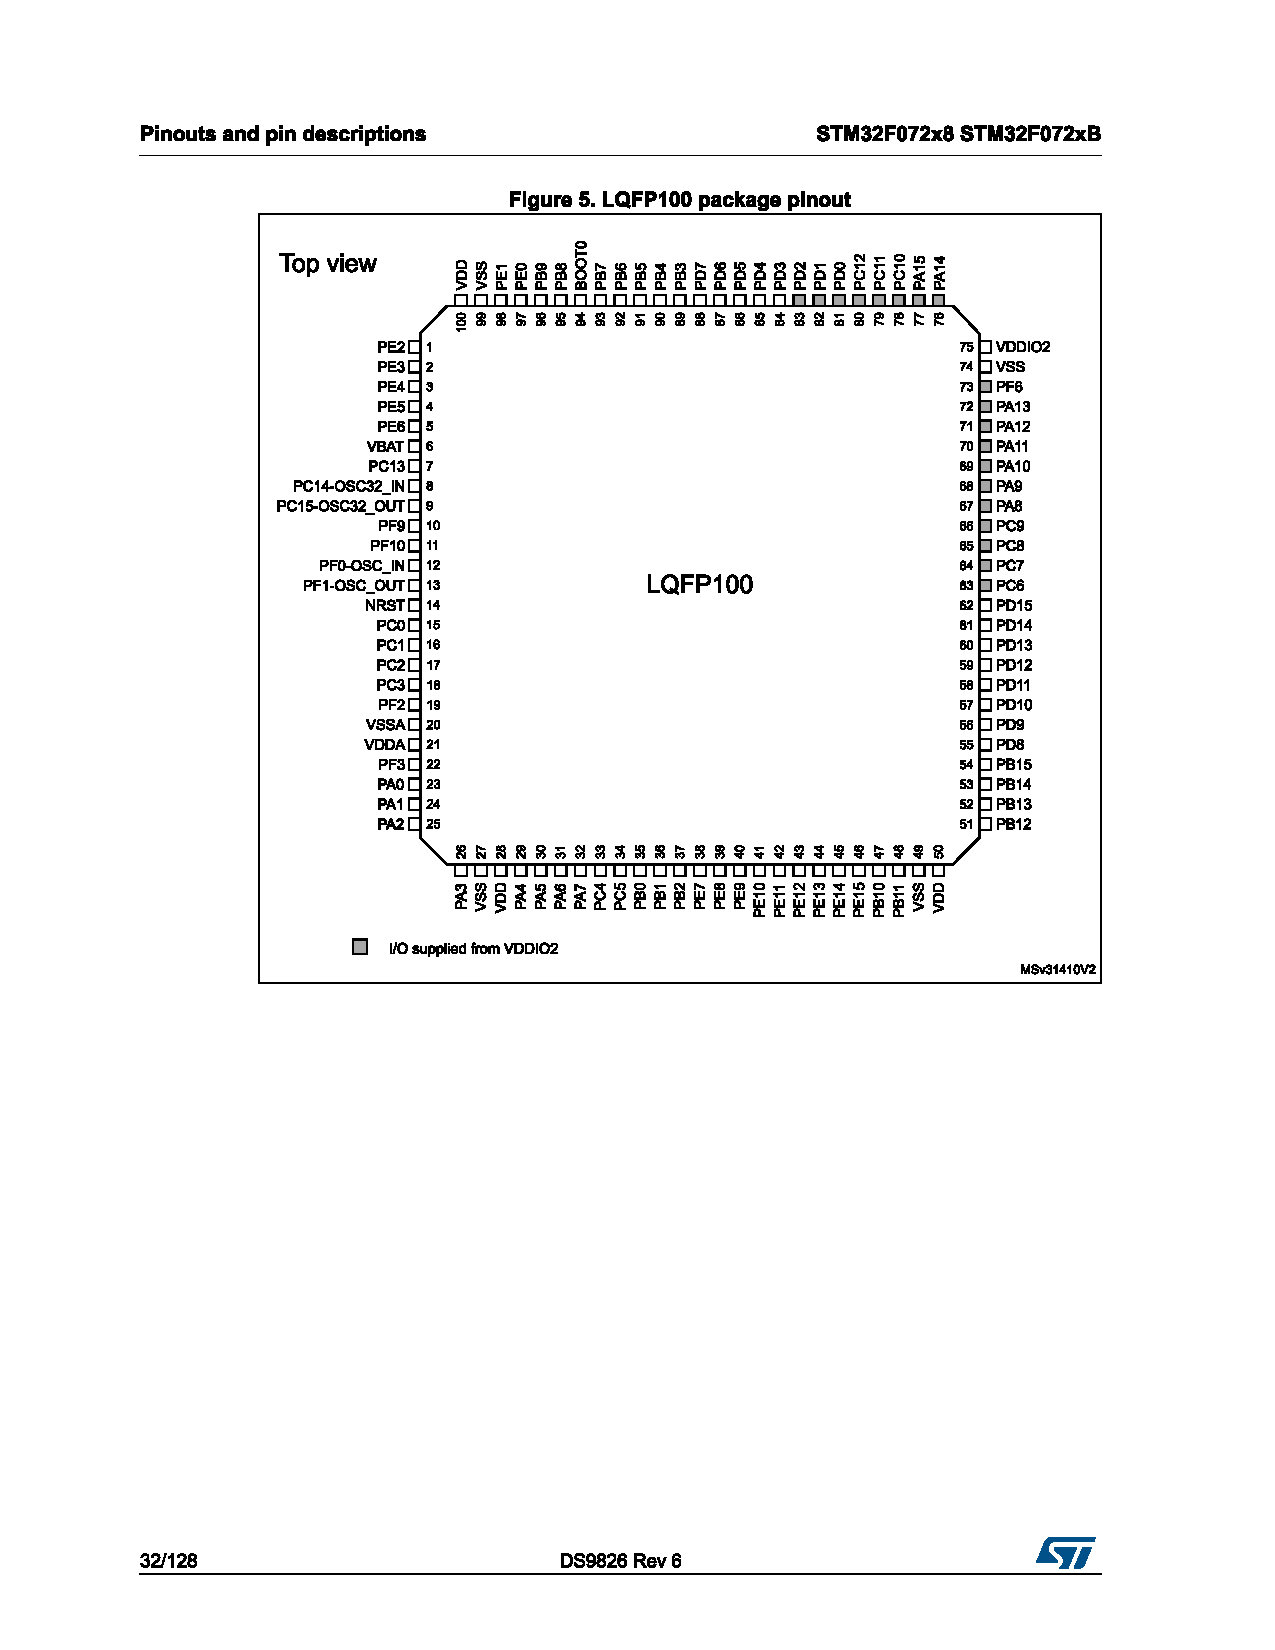
\includepdf[pages=-, scale=0.8, pagecommand={}]{stm32f072cb.pdf}

\newpage

\subsubsection{USB Hub}

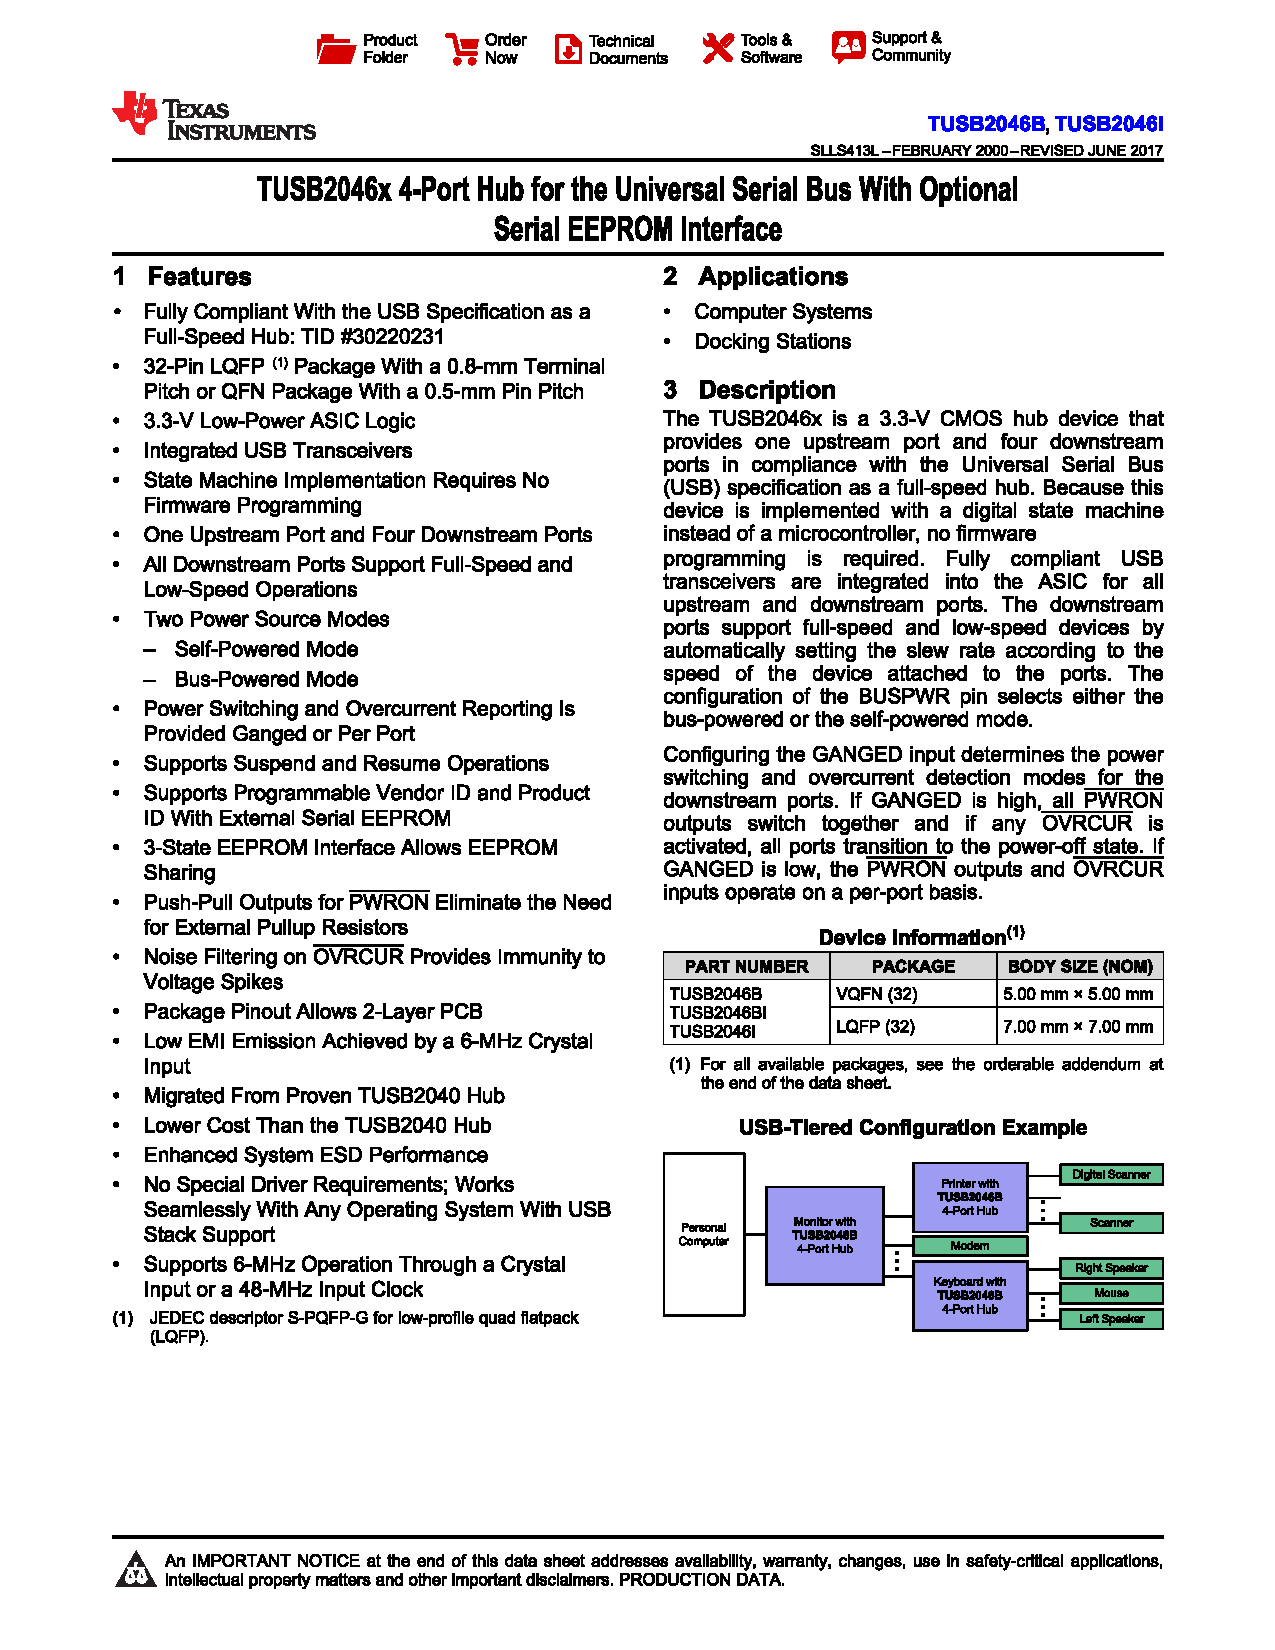
\includepdf[pages=-, scale=0.8, pagecommand={}]{USB Hub.pdf}

\subsubsection{Signal Quality Analysis}

\subsubsection{Saftey/Electrical Hazard Checklist}

\subsubsection{Accuracy Certification}

\newpage

\subsection{Appendix D: Software}
%\begin{enumerate}[noitemsep]
   % \item Flowcharts: An overall flowchart will begin this section. Detailed flowcharts will be done for each individual routine. Each flowchart will be given a descriptive title. The title should be centered at the top of the page. On the line below the title, centered and enclosed in parenthesis, will appear a reference to the corresponding line numbers or page in the software listing where this code can be found. Circles containing an alpha designator will be used to show connectivity between portions of flowcharts. A to/from page number will be placed next to the circle to aid in tracing the flow between pages. Pseudo-code may be used in place of flowcharts for computational code, but not for control or input/output code.
   % \item Program Listings: High Level or Machine: Compressed printing can be used. All programs must have enough comments so that a reviewer can gain insight into the purpose of the program elements.
%\end{enumerate}

\subsection{Appendix E: Resource Expenditure Analysis}
%\begin{enumerate}[noitemsep]
   % \item Cost Analysis: This appendix consists of a list of parts grouped under general headings along with the total price. In narrative form, discuss the nature of any cost overrun, if you are more than 10\% over your estimated cost.
   % \item Labor Hour Analysis: This appendix will contain a breakdown of the hours spent in the development of the hardware and the software. Besides these two main areas, attempt to sub divide it into specific areas as basic research, requisition of parts, testing hardware, testing software, debugging hardware/software, writing the report, etc.
   % \item Parts List: This appendix will contain a listing, in reference designation alpha numeric order, of all the parts used. All parts which do not have a reference designation will be listed in alpha numeric order under a heading of miscellaneous items. Use of the parts list documentation of the schematic capture part of the ORCAD program is recommended.
   % \item Other Resources: Include in this appendix things like funding supplied by others, review time done by others, etc.

\subsubsection{Cost Analysis}

The total material cost for the Harm Drone project was approximately \$326.43, well within the original \$420 project budget. No cost overruns exceeding 10\% occurred. Cost efficiency was maintained through early part procurement and iterative prototyping.

\begin{itemize}
    \item \textbf{Microcontroller and Memory:}
    \begin{itemize}
        \item STM32F072CBT6 Microcontroller – \$3.93
        \item EEPROM Memory – \$0.46
        \item SRAM Memory – \$3.19
        \item SD Card - \$1.28
        \item USB HUB - \$3.41
        \item USB Ports - \$2.22
    \end{itemize}
    \item \textbf{Power System:}
    \begin{itemize}
        \item LMR51430 Buck Converter – \$1.30
        \item XC6210 LDO Regulator – \$1.31
        \item XT60-M - \$1.60
        \item Battery - \$39.99
    \end{itemize}
    \item \textbf{Sensors:}
    \begin{itemize}
        \item Yoctopuce USB Sensors (3x) – \$103.15
        \item USB Temperature Probe – \$10.90
    \end{itemize}
    \item \textbf{Other:}
    \begin{itemize}
        \item 3D-Printed Enclosure – \$10.00
        \item PCB Fabrication – \$119.93
        \item LEDs - \$0.42
        \item Switch - \$0.76
        \item Button - \$1.05
        \item Miscellaneous Passive Components – \$27.55
    \end{itemize}
\end{itemize}

\subsubsection{Labor Hour Analysis}

The estimated total labor effort was approximately 1350 hours across hardware and software design and development. The breakdown is as follows:

\begin{center}
\begin{tabular}{|l|c|}
\hline
\textbf{Task} & \textbf{Hours Spent} \\
\hline
Basic Research and Planning & 400 \\
Parts Requisition and Procurement & 20 \\
Hardware Design (PCB and Enclosure) & 200 \\
Software and Firmware Development & 300 \\
Hardware Assembly and Integration & 100 \\
Testing and Debugging Hardware & 100 \\
Testing and Debugging Software & 150 \\
Final Report Writing and Presentation Preparation & 80 \\
\hline
\textbf{Total} & 1350 \\
\hline
\end{tabular}
\end{center}

\subsubsection{Parts List}

\textbf{Reference Designated Components:}

\begin{itemize}
    \item \textbf{C1, C2, C3, C5, C6, C8, C9, C10, C12, C15, C16, C20, C21} – 0.1\,$\mu$\text{F} Capacitor (0805)
    \item \textbf{C4} – 10\,nF Capacitor (0805)
    \item \textbf{C11, C13, C7} – 4.7\,$\mu$\text{F} Capacitor (0805)
    \item \textbf{C14, C17} – 10\,$\mu$\text{F} Capacitor (0805)
    \item \textbf{C18, C19, C29} – 1\,$\mu$\text{F} Capacitor (0805)
    \item \textbf{C22, C23} – 22\,$\mu$\text{F} Capacitor (0805)
    \item \textbf{C24, C25, C26} – 3.2\,$\mu$\text{F} Capacitor (0805)
    \item \textbf{C27, C28} – 47\,pF Capacitor (0805)
    \item \textbf{C30, C31} – 27\,pF Capacitor (0805)
    \item \textbf{C32, C33} – 22\,pF Capacitor (0805)

    \item \textbf{D1} – PWM LED Indicator (PWM\_LED)
    
    \item \textbf{IC1} – STM32 Microcontroller (Microcontroller)
    \item \textbf{IC2} – USB Hub Controller (USB-HUB)
    \item \textbf{IC3} – LDO Voltage Regulator (LDO)
    \item \textbf{IC4} – SRAM Memory (SRAM)
    
    \item \textbf{J2, J3} – Dual USB Ports (2-Port USB)
    \item \textbf{J4} – XT60 Power Connector (XT60-M)
    \item \textbf{J5} – SD Card Socket (SDCard)
    
    \item \textbf{L1} – 6.8\,$\mu$H Inductor (Inductor)
    
    \item \textbf{R1, R2, R3, R4, R5, R6, R7, R8, R21, R25, R26, R32, R33} – 27\,$\Omega$ Resistors (0805)
    \item \textbf{R9, R10, R11, R12, R13, R14, R15, R16} – 15\,k$\Omega$ Resistors (0805)
    \item \textbf{R17} – 100\,k$\Omega$ Resistor (0805)
    \item \textbf{R18} – 13.7\,k$\Omega$ Resistor (0805)
    \item \textbf{R19, R20, R22, R23, R24} – 10\,k$\Omega$ Resistors (0805)
    \item \textbf{R27, R28} – 270\,$\Omega$ Resistors (0805)
    \item \textbf{R29, R30} – 2.5\,k$\Omega$ Resistors (0805)
    \item \textbf{R34, R35, R36} – 1.5\,k$\Omega$ Resistors (0805)

    \item \textbf{RXLED1, TXLED1} – Status LEDs (LEDC2012X110N, SM0805UBWC)
    
    \item \textbf{S1, S2} – Tactile Pushbutton Switches (SW\_JS102011SAQN)
    
    \item \textbf{U1} – LMR51430 Buck Converter (SOT-23-6)
    \item \textbf{U2} – EEPROM Memory (EEPROM)
    
    \item \textbf{USB-C1} – USB Connector (GCT\_USB4110GFA)
    \item \textbf{USB2UART1} – USB to UART Bridge (FT231XS-R, SSOP-20)
    
    \item \textbf{Y1} – Oscillator Crystal (ECS-060-20-4X, XTAL\_ECS-160-20-4X)
\end{itemize}

\textbf{Miscellaneous Items:}
\begin{itemize}
    \item 3D-Printed PLA Enclosure
    \item MicroSD Card (≥4GB, FAT32 formatted)
    \item Yoctopuce USB Sensors (3x)
    \item USB Temperature Sensor
    \item Power Cable with XT60 Connector
\end{itemize}


\subsubsection{Other Resources}

Funding and technical support for the Harm Drone project were provided by the University of Nebraska’s Electrical and Computer Engineering Department. Review and project sponsorship were provided by Dr. Andrew Harms. Technical instruction on PCB design and USB communication was provided by Dr. Hamid Sharif, and engineering project management guidance was provided by Professor Herbert Detloff.

%\end{enumerate}

\subsection{Appendix F: Individual Student Outcomes Appendices}
\subsubsection{Appendix F1: Carter Brehm}
\subsubsection{Appendix F2: Toby Heinemann}
\subsubsection{Appendix F3: Camryn Klintworth}
\subsubsection{Appendix F4: Michael Maline}
%Each member of the team is responsible for an individual appendix (F1, F2, F3, [F4]) that includes evidence that each member of the team has met ABET Criterion 3, 1) through 7), student outcomes. These can be organized as you wish, but they MUST BE ORGANIZED, not just a collection of notes and miscellaneous course work. Identify each of the 7 outcomes and your supporting evidence.

%%%%%%%%%%%%%%%%%%%%%%%%%%%%%%%%%%%%%%%%%%%%%%%%%%%%%%%%%%%%%%%%%%%%%%%%%%
%                    Report General Guidelines                           %
%%%%%%%%%%%%%%%%%%%%%%%%%%%%%%%%%%%%%%%%%%%%%%%%%%%%%%%%%%%%%%%%%%%%%%%%%%
%\section*{Report General Guidelines}
%\begin{itemize}[noitemsep]
   % \item Be sure to introduce and summarize each section.
   % \item Always write general to specific in each section.
   % \item Do not write chronologically. (a technical report is not a story or a novel)
   % \item Use section and subsection titles.
   % \item Make sure that subsections follow each other in a logical progression.
   % \item Number each page.
   % \item Use bulleted or enumerated lists rather than lengthy textual discussion of requirements, subsystems, etc.
%\end{itemize}
%\begin{itemize}[noitemsep]
   % \item Technical reports only contain Figures and Tables.
   % \item Refer to graphs as figures, photos as figures, small code segments as figures, etc.
   % \item Figures and tables are NOT to be hand sketched.
   % \item Figures and tables should be used to supplement the discussion.
   % \item Always introduce a figure or table in the text and never place a figure or table in the text that is not discussed.
   % \item Discuss the meaning and significance of the table or figure.
   % \item Be sure to highlight the fine points and structure.
   % \item Figures and tables should be located in the body of the text, AFTER they are introduced in the text.
   % \item It is often appropriate to pull out small segments of code from a main program or to write pseudo-code to describe an algorithm or major point of the project. This is considered a figure and should be titled and numbered as such.
   % \item If a group of figures or a long table or code listing takes up too much space, locate them in an appendix.
   % \item Figures and tables can be located at the end of the text, but it is less convenient for the reader.
   % \item Figure titles and numbering: Figures should be numbered consecutively in the report. Every figure must have a descriptive title located immediately below the figure.
   % \item Table titles and numbers: Tables should be numbered consecutively in the report. Every table must have a descriptive title located above or below the table.
  % \end{itemize}

\quickfigure{images/PCB-design-layout.png}{15cm}{PCB Design Layout}{pcb-design-layout}

% todo: the silk screen and drill chart do not match the current PCB design layout above
\quickfigure{images/drill-chart.png}{15cm}{Drill Chart}{drill-chart}

\quickfigure{images/silk-screen.png}{15cm}{Silk Screen}{silk-screen}

\quickfigure{images/right-side-of-PCB-casing.png}{15cm}{Right Side View of PCB Casing}{right-side-view-pcb-casing}

\quickfigure{images/bottom-side-of-PCB-casing.png}{15cm}{Bottom Side of PCB Casing}{bottom-side-pcb-casing}

\quickfigure{images/front-view-of-PCB-casing.png}{15cm}{Front View of PCB Casing}{front-view-pcb-casing}

\quickfigure{images/top-view-PCB-casing-open.png}{15cm}{Top Side View of the PCB Casing}{top-side-view-pcb-casing}

\quickfigure{images/top-front-view-PCB-casing-open.png}{15cm}{Top Front View of the PCB Casing}{top-front-view-pcb-casing}

\quickfigure{images/PCB-CAD-drawing.png}{15cm}{PCB CAD Casing}{pcb-cad-casing}

\quickfigure{images/initial-PCB-footprint-layout.png}{15cm}{Initial PCB Footprint Layout}{initial-pcb-footprint-layout}

%\section*{References}
%Use the IEEE format for reference style. List all references used in the report. All references should include author, title, journal or magazine title (if a journal article), publisher, page number, date. Below are sample references from a conference proceeding paper [1], book [2], journal article [3], Ph.D. dissertation [4], technical specification [5], and web page.
\clearpage
\begin{thebibliography}{99}

\bibitem{parrot2021ardrone}
Parrot, \emph{AR.Drone 2.0 User Guide}, Parrot SA, Sept. 2021. [Online]. Available: \url{https://www.parrot.com/assets/s3fs-public/2021-09/ar.drone2_user-guide_uk.pdf}

\bibitem{parrot2023anafi}
Parrot, \emph{Anafi USA Datasheet}, Parrot SA, 2023. [Online]. Available: \url{https://www.parrot.com/files/s3fs-public/2023-07/parrot-anafi-usa.pdf}

\bibitem{st2023stm32}
STMicroelectronics, ``STM32F072CB Datasheet,'' STMicroelectronics, 2023. [Online]. Available: \url{https://www.st.com/resource/en/datasheet/stm32f072cb.pdf}

\bibitem{ftdi2023ft231x}
FTDI Chip, ``FT231X Full Speed USB to Full Handshake UART,'' FTDI, 2023. [Online]. Available: \url{https://www.ftdichip.com/Support/Documents/DataSheets/ICs/DS_FT231X.pdf}

\bibitem{ti2023tusb}
Texas Instruments, ``TUSB2046I 3.3-V 4-Port USB Hub,'' Texas Instruments, 2023. [Online]. Available: \url{https://www.ti.com/lit/ds/symlink/tusb2046i.pdf}

\bibitem{onsemi2023cat}
ON Semiconductor, ``CAT25160 16-Kb SPI Serial CMOS EEPROM,'' ON Semiconductor, 2023. [Online]. Available: \url{https://www.onsemi.com/pdf/datasheet/cat25160-d.pdf}

\bibitem{issi2023sram}
ISSI Integrated Silicon Solution, Inc., ``IS62WVS2568GBLL 256K x 8 Low Voltage, Ultra Low Power CMOS Static RAM,'' ISSI, 2023. [Online]. Available: \url{https://www.issi.com/WW/pdf/62-65WV2568GBLL.pdf}

\bibitem{samesky2023msd}
Same Sky, \emph{MSD-12-A microSD Card Connector Datasheet}, 2023. [Online]. Available: \url{https://www.sameskydevices.com/product/resource/msd-12-a.pdf}

\bibitem{microchip2023sram}
Microchip Technology Inc., ``23LC1024 1 Mbit SPI Serial SRAM,'' Microchip Technology, 2023. [Online]. Available: \url{https://ww1.microchip.com/downloads/en/DeviceDoc/25142A.pdf}

\bibitem{ti2023stepdown}
Texas Instruments, ``LMR51430 4.3-A, 36-V, 2.1-MHz Synchronous Step-Down Converter,'' Texas Instruments, 2023. [Online]. Available: \url{https://www.ti.com/lit/ds/symlink/lmr51430.pdf}

\bibitem{torex2023ldo}
Torex Semiconductor Ltd., ``XC6210 Series 700mA High-Speed LDO Regulators,'' Torex Semiconductor, 2023. [Online]. Available: \url{https://www.torexsemi.com/file/xc6210/XC6210.pdf}

\bibitem{speasl2022payload}
J. Speasl, M. Patterson, and M. Roberts, ``Removable sensor payload system for unmanned aerial vehicle performing media capture and property analysis,'' U.S. Patent 11,501,483 B2, Nov. 15, 2022. [Online]. Available: \url{https://patents.google.com/patent/US11501483B2/en}

\bibitem{kendall2022remote}
R. Kendall, R. Jonkman, and S. Talaber, ``High-Altitude Airborne Remote Sensing,'' U.S. Patent Application 2022/0404273 A1, Dec. 22, 2022. [Online]. Available: \url{https://patents.google.com/patent/US20220404273A1/en}

\bibitem{bart2019autodrone}
G. F. Bart and E. Caglayan, ``Autonomous drone with image sensor,'' U.S. Patent 10,462,366 B1, Oct. 29, 2019. [Online]. Available: \url{https://patents.google.com/patent/US10462366B1/en}

\bibitem{microchip2023atmega}
Microchip Technology Inc., ``ATmega32U4 Datasheet,'' Microchip Technology Inc., 2023. [Online]. Available: \url{https://ww1.microchip.com/downloads/en/DeviceDoc/Atmel-7766-8-bit-AVR-ATmega16U4-32U4_Datasheet.pdf}

\bibitem{silabs2023cp2102}
Silicon Labs, ``CP2102 USB to UART Bridge Controller,'' Silicon Labs, 2023. [Online]. Available: \url{https://www.silabs.com/documents/public/data-sheets/cp2102.pdf}

\bibitem{mps2023mp2315}
Monolithic Power Systems, ``MP2315 2.5A, 24V, 1.4MHz Step-Down Converter,'' MPS, 2023. [Online]. Available: \url{https://www.monolithicpower.com/en/documentview/productdocument/index/version/2/document_type/Datasheet/lang/en/sku/MP2315/document_id/100/}

\bibitem{terminus2023fe11s}
Terminus Technology Inc., ``FE1.1S USB 2.0 Hub Controller,'' Terminus Technology, 2023. [Online]. Available: \url{http://www.terminus.com.tw/pdf/FE1.1s.pdf}

\bibitem{ams2023ams1117}
Advanced Monolithic Systems, ``AMS1117 Datasheet,'' AMS, 2023. [Online]. Available: \url{http://www.advanced-monolithic.com/pdf/ds1117.pdf}

\bibitem{microchip2023at24c256}
Microchip Technology Inc., ``AT24C256 256-Kbit 2-wire Serial EEPROM,'' Microchip Technology, 2023. [Online]. Available: \url{https://ww1.microchip.com/downloads/en/DeviceDoc/doc0336.pdf}

\bibitem{nspe2020}
National Society of Professional Engineers (NSPE), \emph{Code of Ethics for Engineers}, 2020. [Online]. Available: \url{https://www.nspe.org/resources/ethics/code-ethics}

\bibitem{ieee_ethics}
IEEE Global Initiative, \emph{Ethically Aligned Design: A Vision for Prioritizing Human Well-being with Autonomous and Intelligent Systems}, 1st ed., 2019. [Online]. Available: \url{https://ethicsinaction.ieee.org/}

\bibitem{ipc2221}
IPC, \emph{IPC-2221B: Generic Standard on Printed Board Design}, IPC Association, 2012. [Online]. Available: \url{https://shop.ipc.org/IPC-2221B-Redline-2221B-RL-P-0-EN}

\bibitem{rohs}
European Union, \emph{Directive 2011/65/EU on the Restriction of Hazardous Substances (RoHS)}, 2011. [Online]. Available: \url{https://eur-lex.europa.eu/legal-content/EN/TXT/?uri=CELEX:32011L0065}

\bibitem{ear}
U.S. Department of Commerce, Bureau of Industry and Security, \emph{Export Administration Regulations (EAR)}, 2023. [Online]. Available: \url{https://www.bis.doc.gov/index.php/regulations/export-administration-regulations-ear}

\bibitem{ccpa}
State of California Department of Justice, “California Consumer Privacy Act (CCPA),” Mar. 13, 2024. [Online]. Available: \url{https://oag.ca.gov/privacy/ccpa}

\bibitem{ieee1789}
IEEE Standards Association, \emph{IEEE Std 1789-2015: Recommended Practices for Modulating Current in High-Brightness LEDs}, 2015. [Online]. Available: \url{https://standards.ieee.org/standard/1789-2015.html}

\bibitem{goncalves_uav}
D. Gonçalves, A. Pereira, and R. Silva, “Sustainability in UAVs: Bio-Based and Recycled Composites,” \emph{Materials}, vol. 9, no. 4, p. 169, Apr. 2023. [Online]. Available: \url{https://www.mdpi.com/2504-477X/9/4/169}

\bibitem{natureworks_pla}
NatureWorks LLC, \emph{Polylactic Acid (PLA) Bioplastic: Environmental Benefits and Life Cycle Assessment}, 2023. [Online]. Available: \url{https://www.natureworksllc.com/What-is-Ingeo/Why-it-Matters}

\end{thebibliography}

%%%%%%%%%%%%%%%%%%%%%%%%%%%%%%%%%%%%%%%%%%%%%%%%%%%%%%%%%%%%%%%%%%%%%%%%%%
%                              End Document                              %
%%%%%%%%%%%%%%%%%%%%%%%%%%%%%%%%%%%%%%%%%%%%%%%%%%%%%%%%%%%%%%%%%%%%%%%%%%
\end{document}
